%%%%%%%%%%%%%%%%%%%%%%%%%%%%%%%%%%%%%%%%%%%%%%%%%%%%%%%%%%%%%%%%%%%%%%%%%%%%
%%                                                                        %%
%%                 Support de cours Programmation orientée objet                  %%
%%                                                                        %%
%%%%%%%%%%%%%%%%%%%%%%%%%%%%%%%%%%%%%%%%%%%%%%%%%%%%%%%%%%%%%%%%%%%%%%%%%%%%
%% Guillaume Moreau (EC Nantes)
%% création : 21/06/2004
%% dernière modification : 23/06/2004
%% historique :

%% il faut fixer l'URL base pour que les liens relatifs fonctionnent...
%% bizaremment fichu mais c'est comme ça.

\documentclass[allowframebreaks,xcolor=dvipsnames]{beamer}

\mode<presentation>
{
\usetheme{Antibes}
  % or ...

  %\setbeamercovered{transparent}
  % or whatever (possibly just delete it)
}
\useoutertheme{infolines}
\usecolortheme[named=RoyalBlue]{structure}

\uselanguage{french}
\languagepath{french}
\deftranslation[to=french]{definition}{définition}
\deftranslation[to=french]{Definition}{D\'efinition}

\setbeamertemplate{blocks}[rounded][shadow=true]
\setbeamertemplate{navigation symbols}{}
\setbeamertemplate{itemize item}[square]
\setbeamertemplate{itemize subitem}[triangle]

\usepackage[T1]{fontenc}
\usepackage[utf8]{inputenc}
% or whatever

\usepackage[french]{babel}
% or whatever

%% pour afficher le plan à chaque début de section
%\AtBeginSection[]{
%  \begin{frame}{Plan}
%  \tiny \tableofcontents[currentsection, hideothersubsections]
%  \end{frame}
%}


%% tout ce qui est relatifs aux extraits de code
\usepackage{listings}
\usepackage{lstautogobble}
\lstloadlanguages{C++}
\lstset{% paramètres généraux des listings
	language=C++,
	basicstyle=\ttfamily\tiny, %% style général : chasse fixe, taille minimale
	keywordstyle=\color{webgreen}\bfseries, % les mots clés en vert et gras
	stringstyle=\color{blue}, % les chaines de caractères en bleu
	commentstyle=\color{webbrown},
	autogobble
}


\usepackage{myslides}

%\usepackage{times}
\usepackage[T1]{fontenc}
% Or whatever. Note that the encoding and the font should match. If T1
% does not look nice, try deleting the line with the fontenc.


\title[Option RV / IMAGE] % (optional, use only with long paper titles)
{Images de synthèse temps en réel}

\author[G. Moreau]{Guillaume Moreau\\
\texttt{guillaume.moreau@ec-nantes.fr}}
% - Use the \inst{?} command only if the authors have different
%   affiliation.

\institute[Ecole Centrale de Nantes] % (optional, but mostly needed)
{
  Ecole Centrale de Nantes
}

\date % (optional)
{Septembre 2019}

\subject{Images de synthèse temps-réel}


\definecolor{webgreen}{rgb}{0,.5,0}
\definecolor{webbrown}{rgb}{.6,0,0}
\definecolor{* }{rgb}{0,.5,0}
\definecolor{. }{rgb}{.6,0,0}


% Delete this, if you do not want the table of contents to pop up at
% the beginning of each subsection:
\AtBeginSection[]
{
   \begin{frame}
       \frametitle{Plan}
       \tableofcontents[sectionstyle=show/hide,subsectionstyle=show/show/hide]
   \end{frame}
}

\newcommand{\sitem}[1]{\begin{itemize}\item #1\end{itemize}}


\begin{document}

\begin{frame}
  \titlepage
\end{frame}

\begin{frame}[allowframebreaks]{Plan du cours}
  \tableofcontents[hideallsubsections]
  % You might wish to add the option [pausesections]
\end{frame}


% intro et déroulement du cours

\begin{frame}{Contenu du cours}
\begin{columns}
\begin{column}{0.6\textwidth}
\begin{itemize}
\item Modèles utilisés pour la synthèse d'images
\begin{itemize}
\item Synthèse d'images temps réel : le modèle d'OpenGL
\item Quelques idées sur la synthèse d'images hors ligne
\end{itemize}
\item Programmation OpenGL
\item Focus sur les shaders
\item Unity3D
\item Les graphes de scène
\item OpenSceneGraph
\end{itemize}
\end{column}
\begin{column}{0.39\textwidth}
\begin{center}
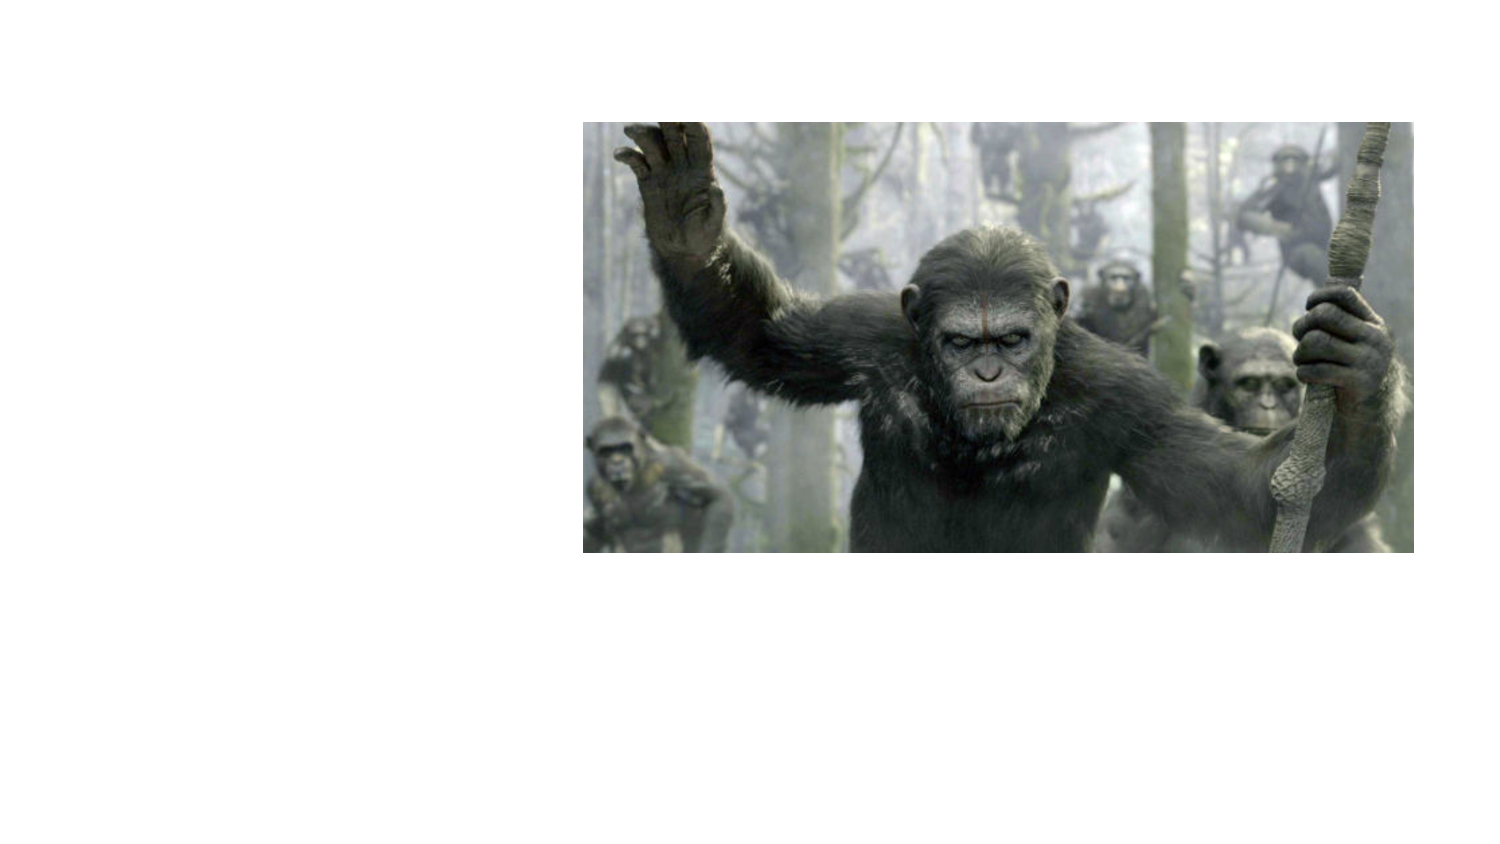
\includegraphics[width=\textwidth]{figs/apes.pdf}
\end{center}
\end{column}
\end{columns}
\end{frame}

\begin{frame}{Introduction}
\begin{center}
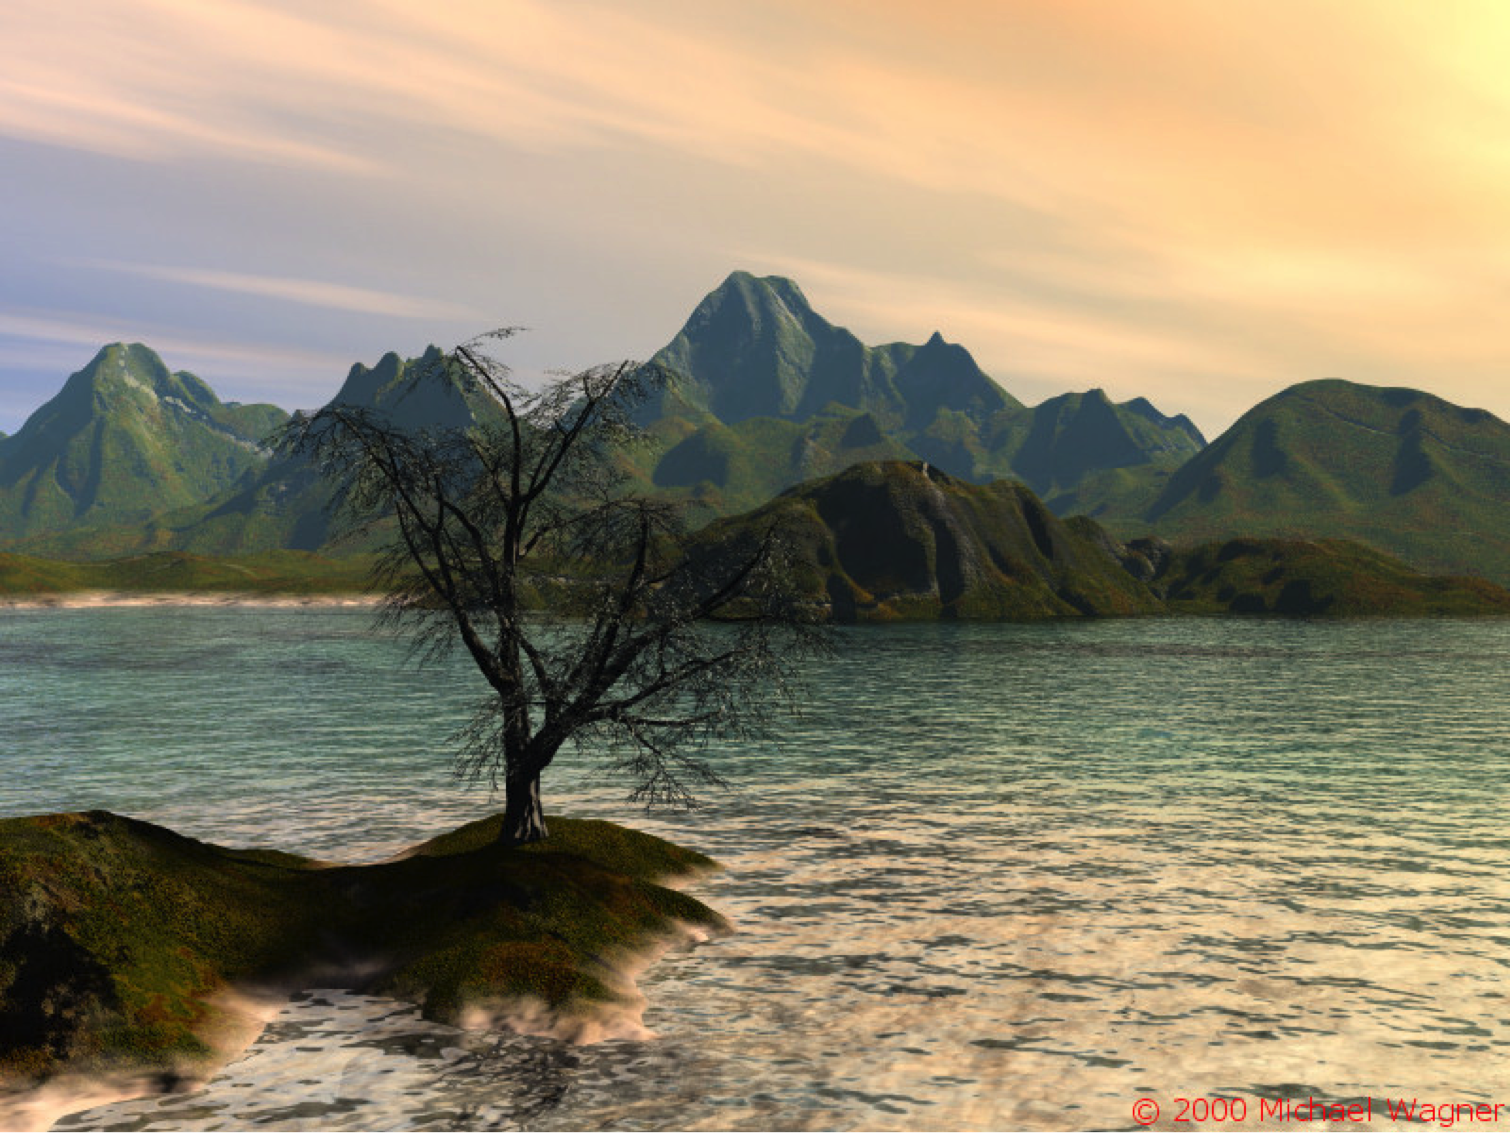
\includegraphics[height=\textheight]{figs/wagner00.png}
\emph{Dawn of the Planet of the Apes, 2014}
\end{center}
\end{frame}

\subsection{Petite histoire de la synthèse d'images}

\begin{frame}{Images de synthèse et cinéma (1/2)}
\begin{itemize}
\item 1976 : première apparition \textit{Future World}
\item 1982 : pendant tout le film \textit{Tron}
\item 1984 : se veut réaliste \textit{Last Star Fighter}
\item 1988 : premier Oscar \textit{Tin Toy}
\item 1989 : avec des êtres vivants \textit{Abyss}
\end{itemize}
\begin{center}
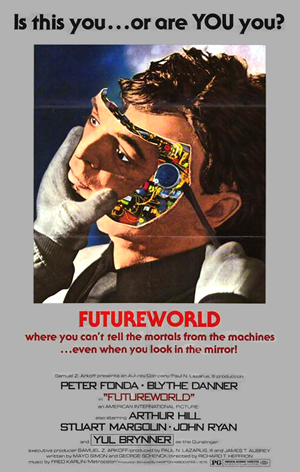
\includegraphics[height=0.28\textheight]{figs/Futureworld.jpg}
\hspace{0.1cm}
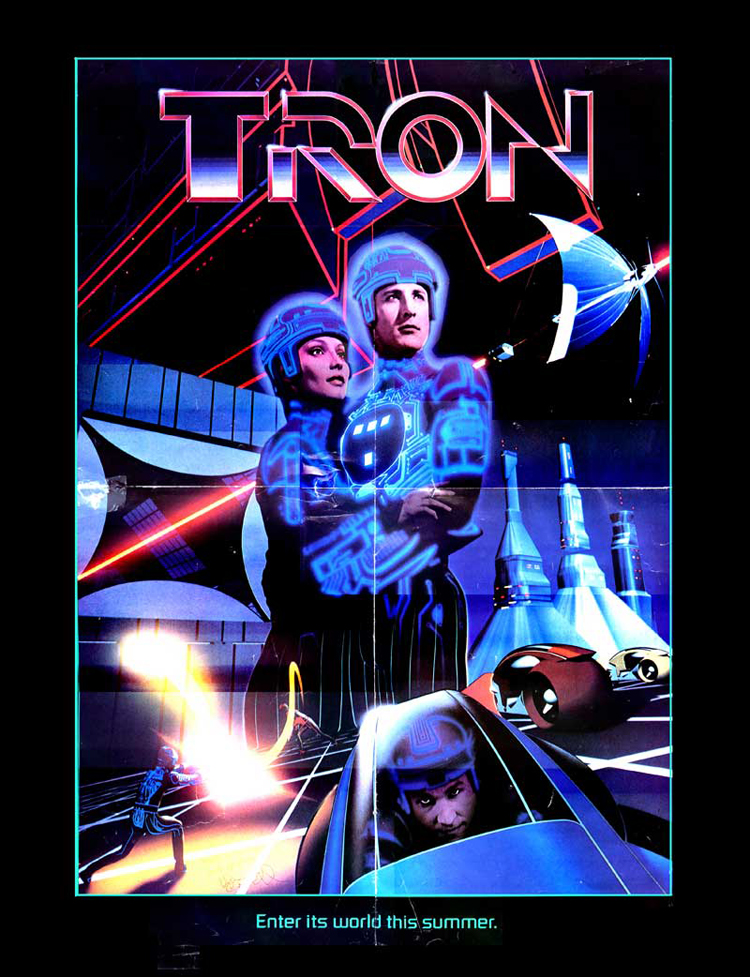
\includegraphics[height=0.28\textheight]{figs/Tron1982.jpg}
\hspace{0.1cm}
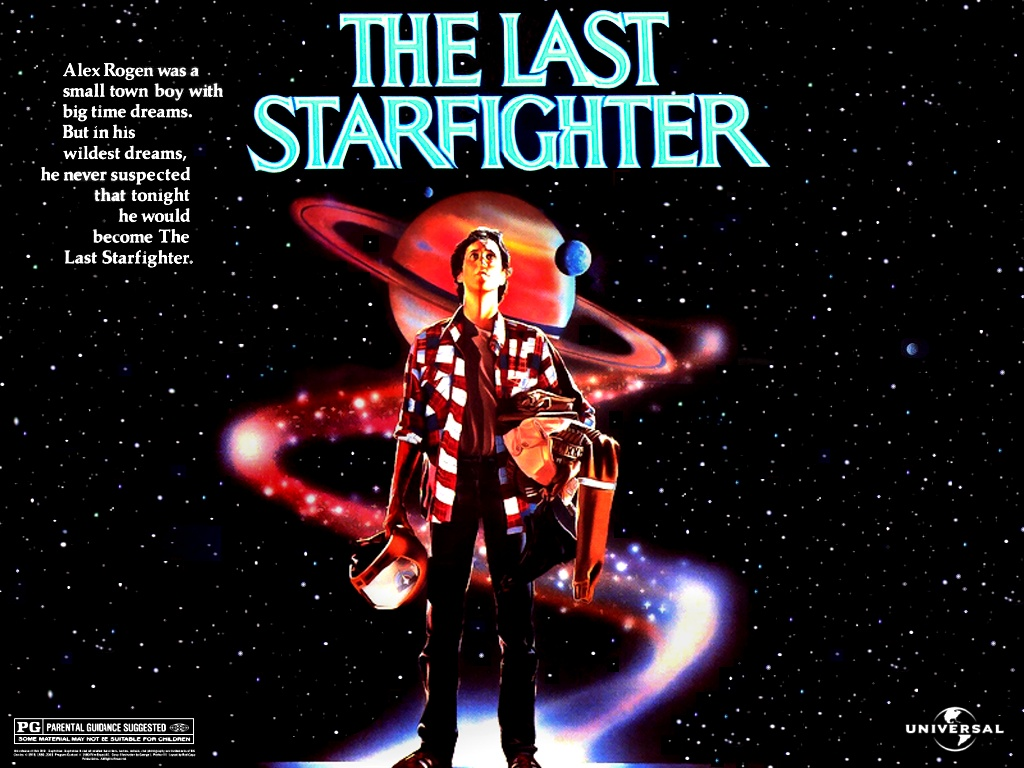
\includegraphics[height=0.28\textheight]{figs/thelaststarfighter.jpg}
\hspace{0.1cm}

\includegraphics[height=0.28\textheight]{figs/tintoy.jpg}
\hspace{0.1cm}
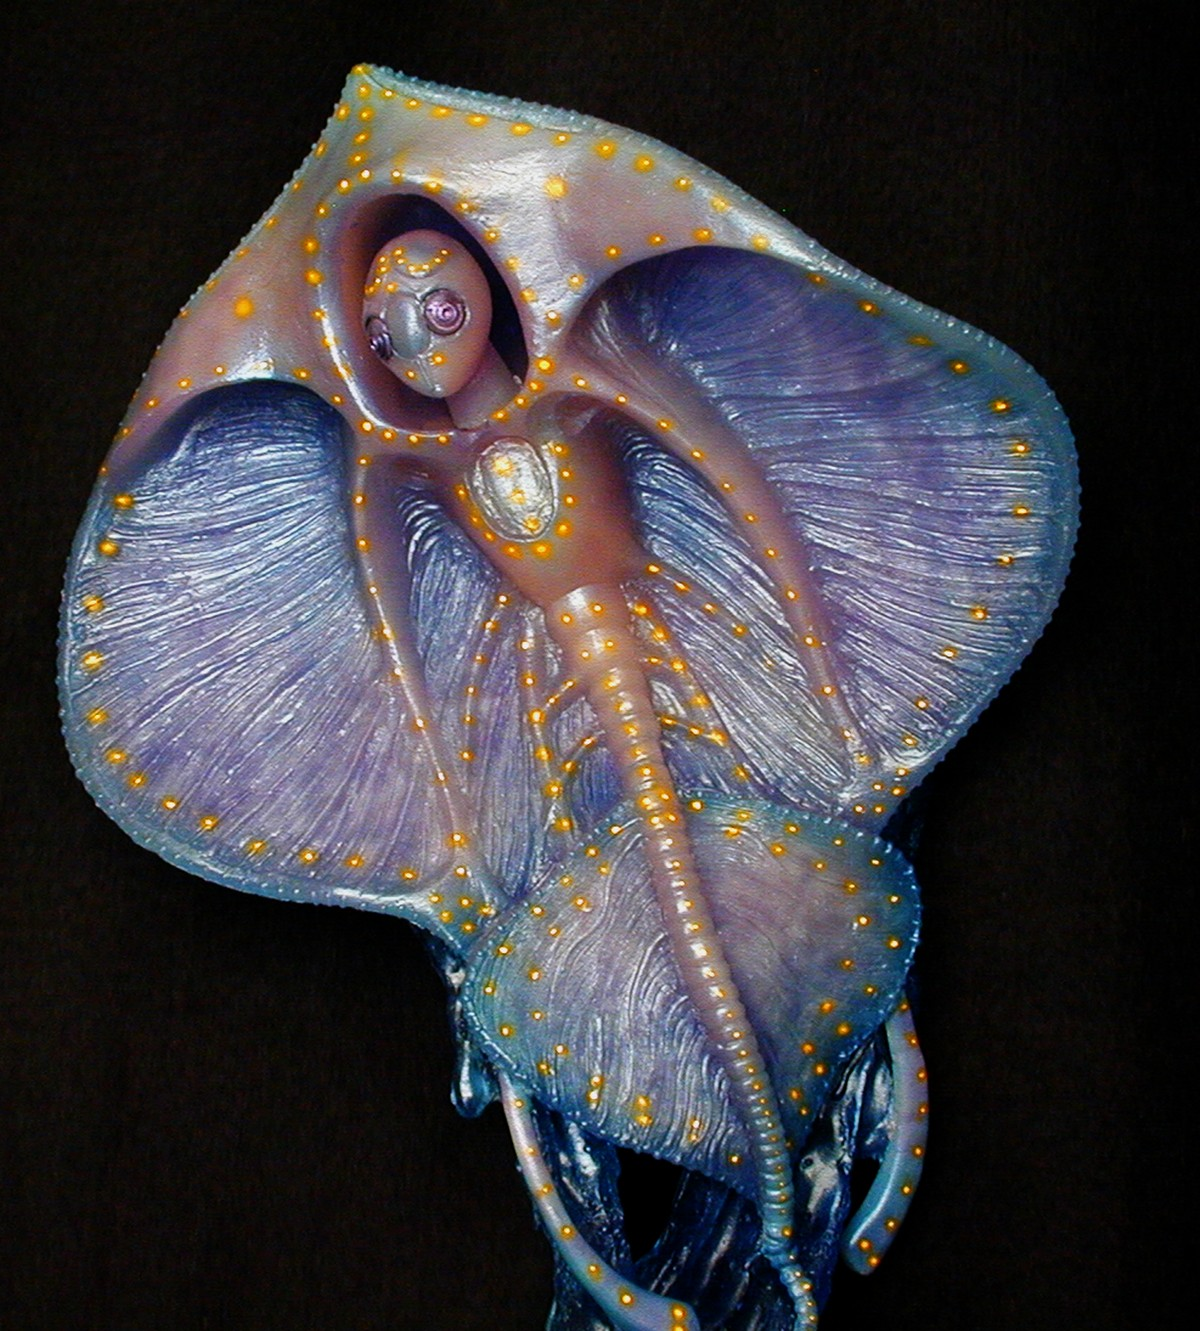
\includegraphics[height=0.28\textheight]{figs/abyss.jpg}
\end{center}
\end{frame}

\begin{frame}{Images de synthèse et cinéma (2/2)}
\begin{itemize}
\item 1993 : premières créatures connues \textit{Jurassic Park}
\item 1982 : doublures d'acteurs \textit{Batman returns}
\item 1984 : 3D de synthèse intégrale \textit{Toy Story}
\item Et ça continue...
\end{itemize}
\begin{center}
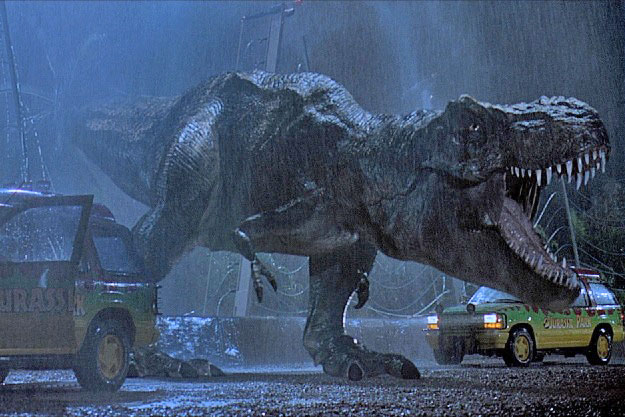
\includegraphics[height=0.28\textheight]{figs/Jurassic-Park.jpg}
\hspace{0.1cm}
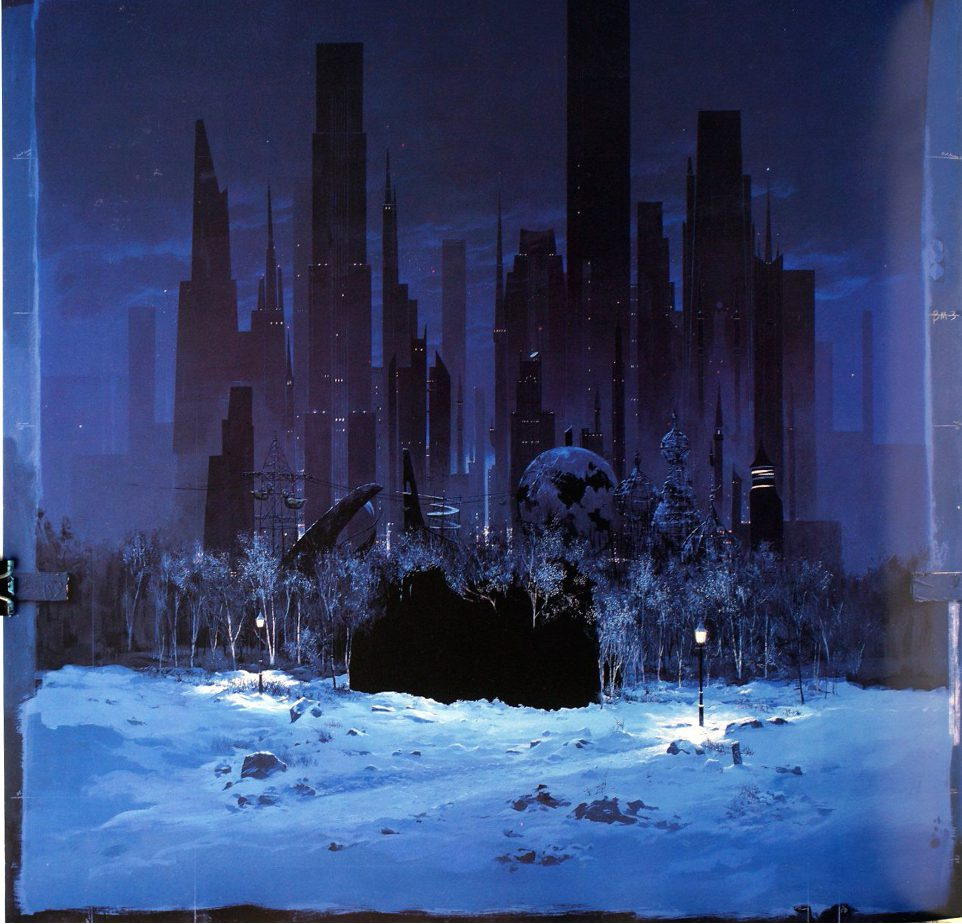
\includegraphics[height=0.28\textheight]{figs/BatmanReturns.jpg}
\hspace{0.1cm}
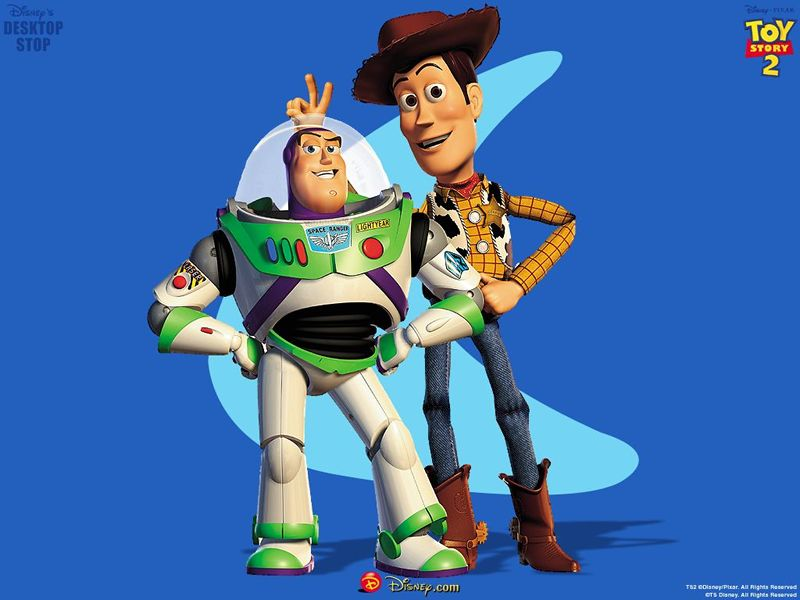
\includegraphics[height=0.28\textheight]{figs/ToyStory.jpg}
\end{center}
\end{frame}

\begin{frame}{Rappel}
\begin{itemize}
\item Dans ce cours, on s'intéresse la plupart du temps à la synthèse d'images en temps réel
\begin{center}
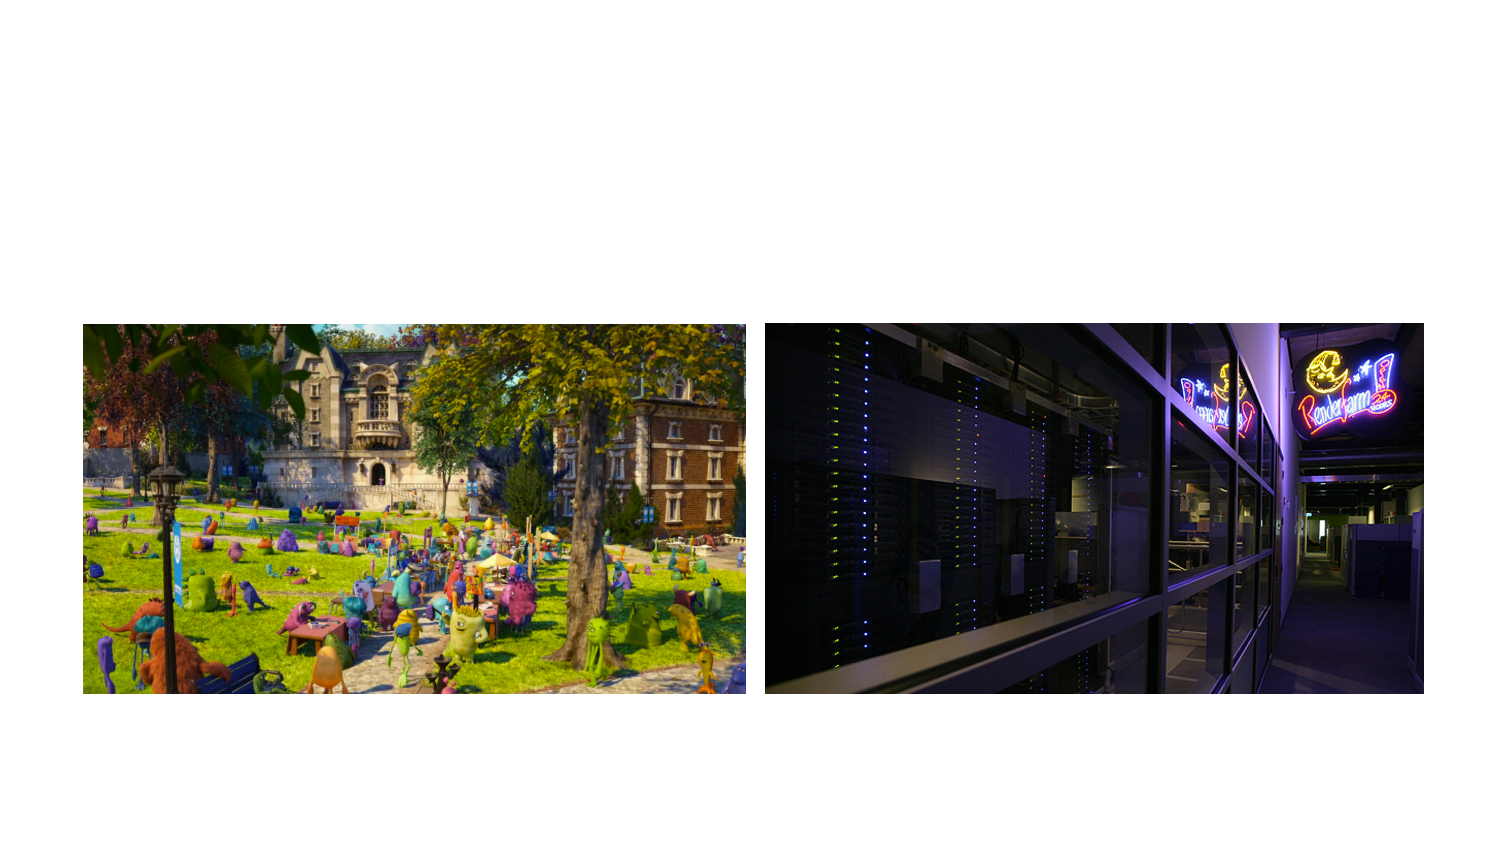
\includegraphics[width=.9\textwidth]{figs/monsters.pdf}
\end{center}
\item 1 image de \textit{Monstres Academy} : 29h de calcul sur une ferme de 24000 c\oe urs !
\end{itemize}
\end{frame}

\begin{frame}{Eléments de bibliographie}
\begin{itemize}
\item Livres
\begin{itemize}
\item Informatique graphique et rendu. B. Péroche, D. Bechmann (Eds). Hermès, 2007.
\item 3D Computer Graphics. A. Watt, Addison-Wesley, 1999. 642 pages !
\item Computer Graphics, Principles and Practice. J. Hughes, A. van Dam, M. McGuire, D. Sklar, J. Foley, S. Feiner, K. Akeley. Addison-Wesley, 2013. 1264 pages. La suite du \textit{Foley et van Dam}.
\end{itemize}
\item Revues scientifiques
\begin{itemize}
\item ACM SIGGRAPH : salon professionnel, conférence scientifique
\item ACM Transactions on Graphics
\end{itemize}
\item Cours en ligne
\begin{itemize}
\item Coursera : \url{https://www.coursera.org/course/interactivegraphics}
\item EdX : \url{https://www.edx.org/course/uc-berkeleyx/uc-berkeleyx-cs-184-1x-foundations-1003}
\item OpenCourseWare \url{http://ocw.mit.edu/courses/electrical-engineering-and-computer-science/6-837-computer-graphics-fall-2012/}
\end{itemize}
\end{itemize}
\end{frame}


\section{Du modèle au rendu}

\subsection{Différents modèles}

\begin{frame}{Définition}
\begin{block}{Définition}
Un écran est un rectangle à deux dimensions, discrétisé en un ensemble de rectangles uniformes appelés \textit{pixels}
\end{block}
\begin{itemize}
\item Conséquence : une \textit{image} est une suite de points de l'écran
\item La synthèse d'images est le calcul des valeurs (couleurs) des éléments de la suite
\item On distingue plusieurs types de rendu
\begin{itemize}
\item Rendu \textit{photo-réaliste} : on cherche à s'approcher de la réalité
\item Rendu \textit{non photo-réaliste} : on s'éloigne délibérément d'un rendu se rapprochant de la réalité
\end{itemize}
\end{itemize}
\begin{center}
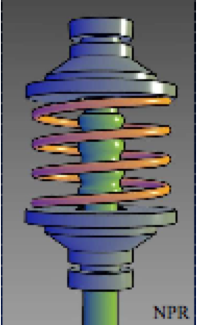
\includegraphics[height=0.25\textheight]{figs/nprcao.png}
\hspace{0.1cm}
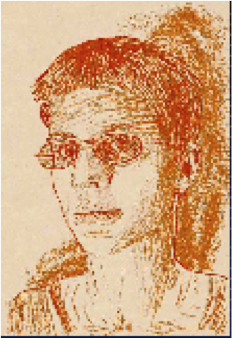
\includegraphics[height=0.25\textheight]{figs/npr-points.png}
\hspace{0.1cm}
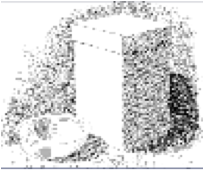
\includegraphics[height=0.25\textheight]{figs/npr-points2.png}
\end{center}

\end{frame}


\begin{frame}{Problématique}
\begin{itemize}
\item Associer à chaque pixel une intensité lumineuse qui dépend de :
\begin{itemize}
\item Des objets de la scène et de leurs propriétés physiques
\item Des sources lumineuses éclairant la scène
\item De la position des objets dans la scène
\item De la caméra virtuelle qui filme la scène
\begin{itemize}
\item position, orientation
\item caractéristiques techniques
\end{itemize}
\end{itemize}
\end{itemize}
\end{frame}

\begin{frame}{Le processus de rendu}
\begin{center}
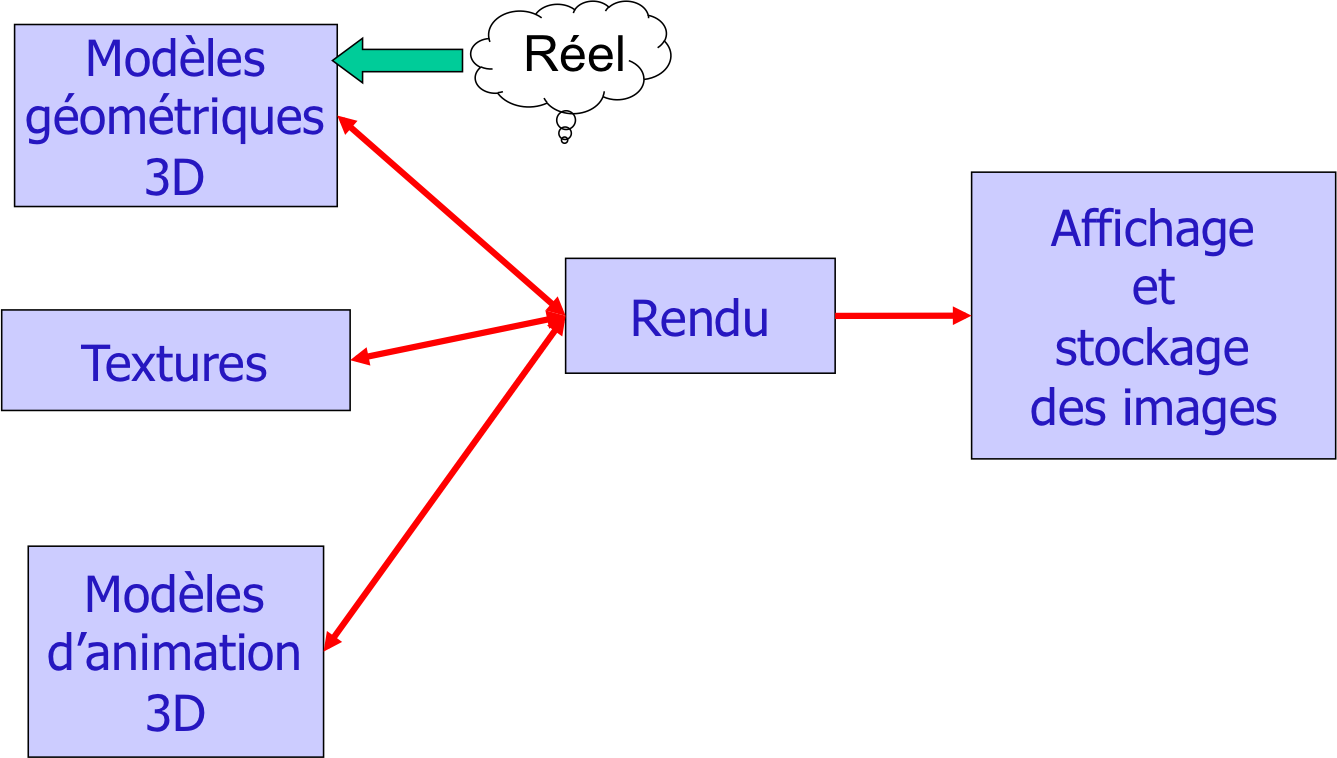
\includegraphics[height=.8\textheight]{figs/rendu.png}
\end{center}
\end{frame}

\begin{frame}{Rendu temps-réel}
\begin{center}
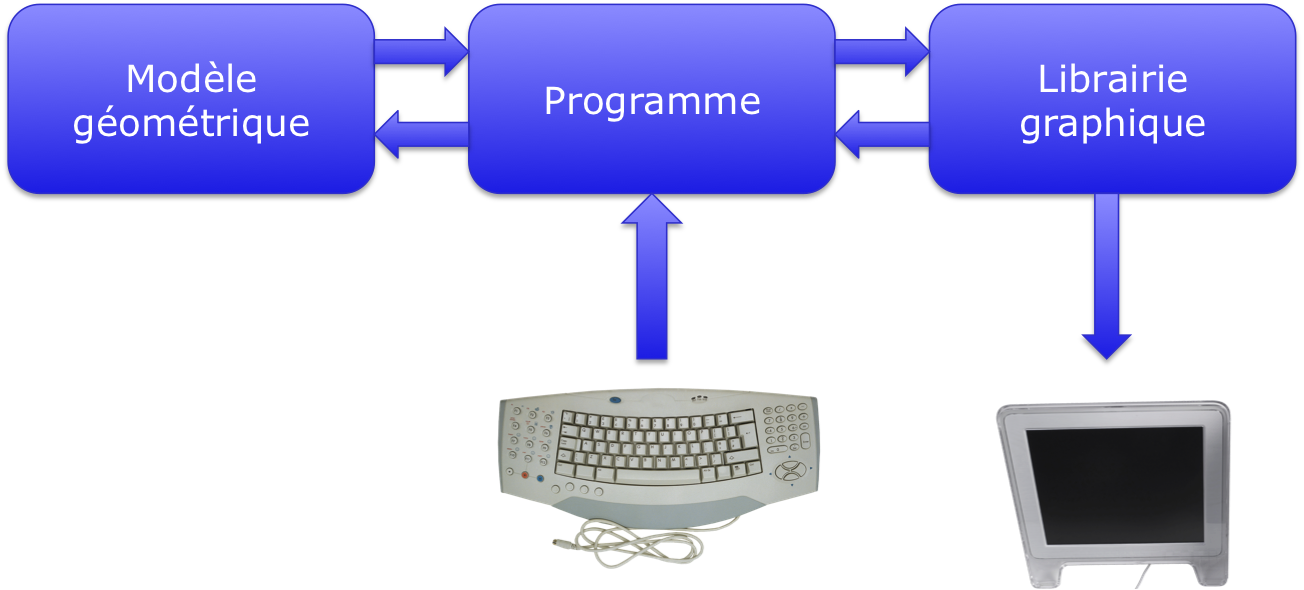
\includegraphics[width=.9\textwidth]{figs/rendurt.png}
\end{center}
\end{frame}

\begin{frame}{Modélisation géométrique}
\begin{center}
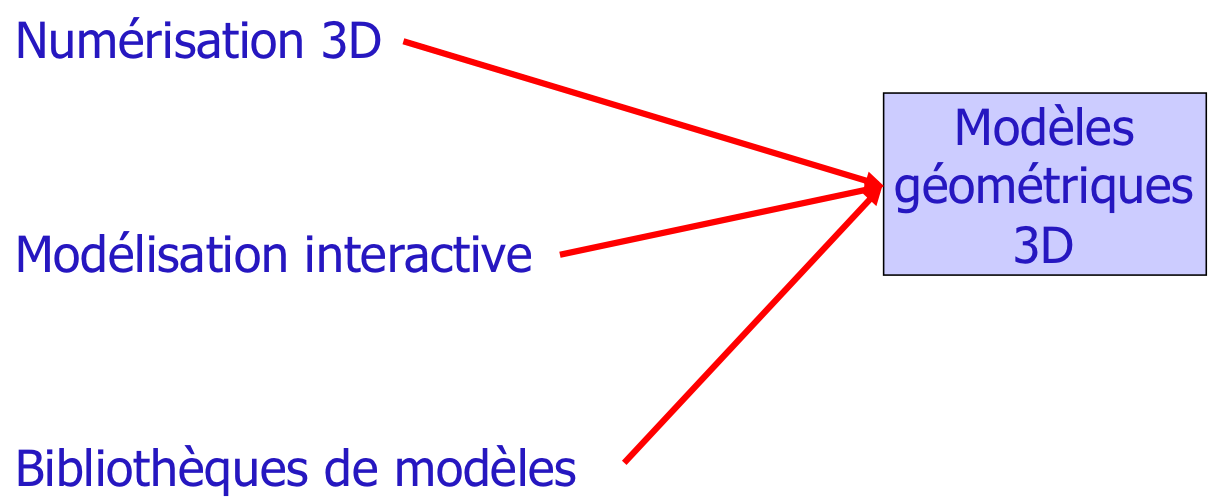
\includegraphics[width=.9\textwidth]{figs/modgeom.png}
\end{center}

\end{frame}

\begin{frame}{Animation}
\begin{center}
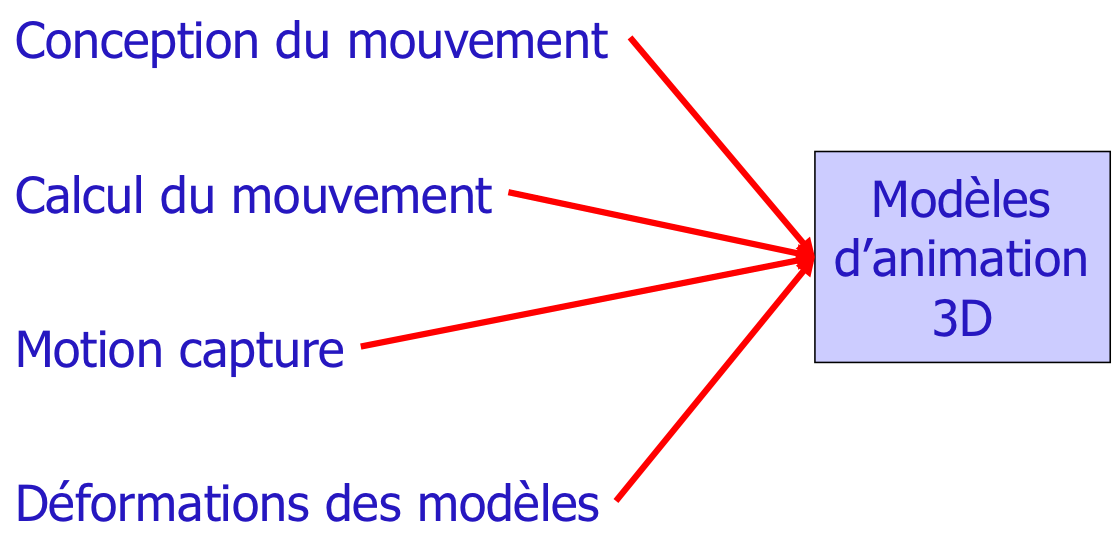
\includegraphics[width=.9\textwidth]{figs/anim.png}
\end{center}

\end{frame}

\begin{frame}{Modèles géométriques}
\begin{center}
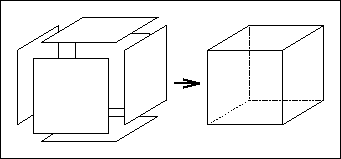
\includegraphics[height=1.8cm]{figs/brep.png}
\end{center}
\begin{itemize}
\item Description des objets
\begin{itemize}
\item Forme
\item Attributs
\item Comportements, propriétés
\end{itemize}
\item Stocké en mémoire par l'application, modifiable par l'application
\item Principe B-Rep (Boundary representation) : un solide est représenté par sa frontière extérieure
\item Plusieurs types de modèles (voir cours GEOMOD3D)
\begin{itemize}
\item Primitives (boites, cônes, sphères)
\item Surfaces triangulées
\item Surfaces de révolution
\item Combinaison de primitives
\end{itemize}
\end{itemize}
\end{frame}

\begin{frame}{Surfaces triangulées}
\begin{columns}
\begin{column}{.6\textwidth}
\begin{itemize}
\item Ensemble de triangles obtenus par
\begin{itemize}
\item construction
\item \textit{tessellation}
\end{itemize}
\item Normale au triangle
\begin{itemize}
\item définit l'intérieur/extérieur
\item Souvent implicite
\end{itemize}
\end{itemize}
\end{column}
\begin{column}{.39\textwidth}
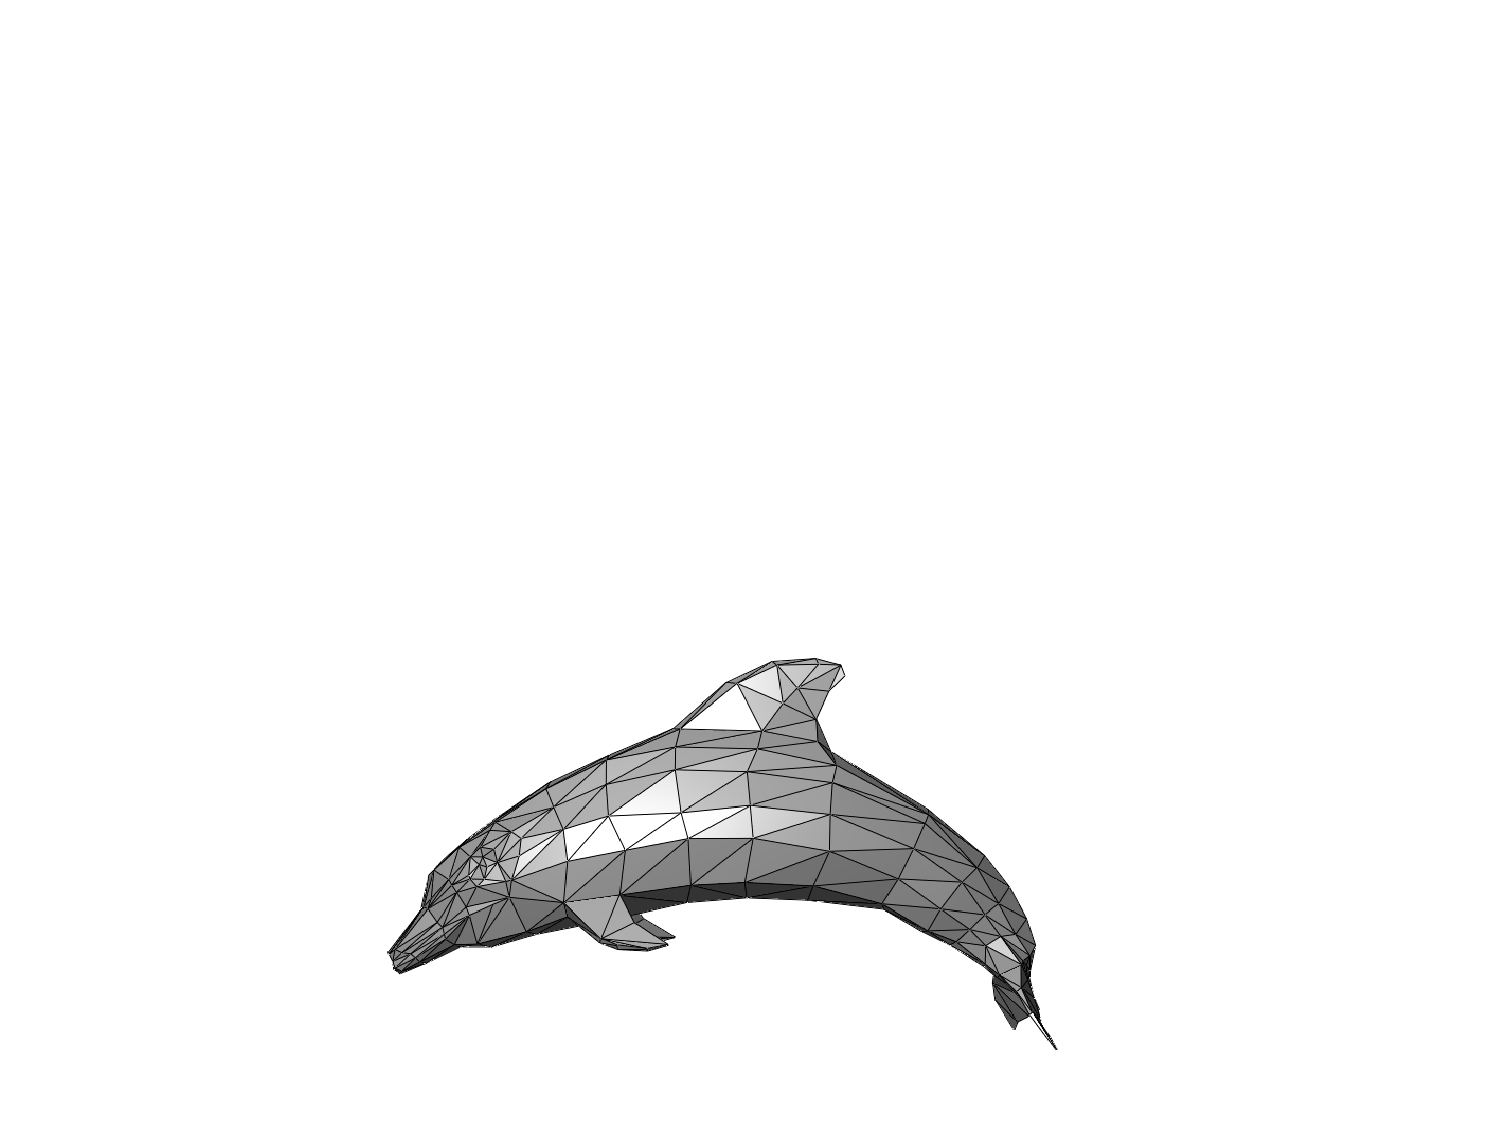
\includegraphics[width=\textwidth]{figs/dauphin.pdf}
\end{column}
\end{columns}
\end{frame}

\begin{frame}{Quelle quantité de triangles ?}
\begin{center}
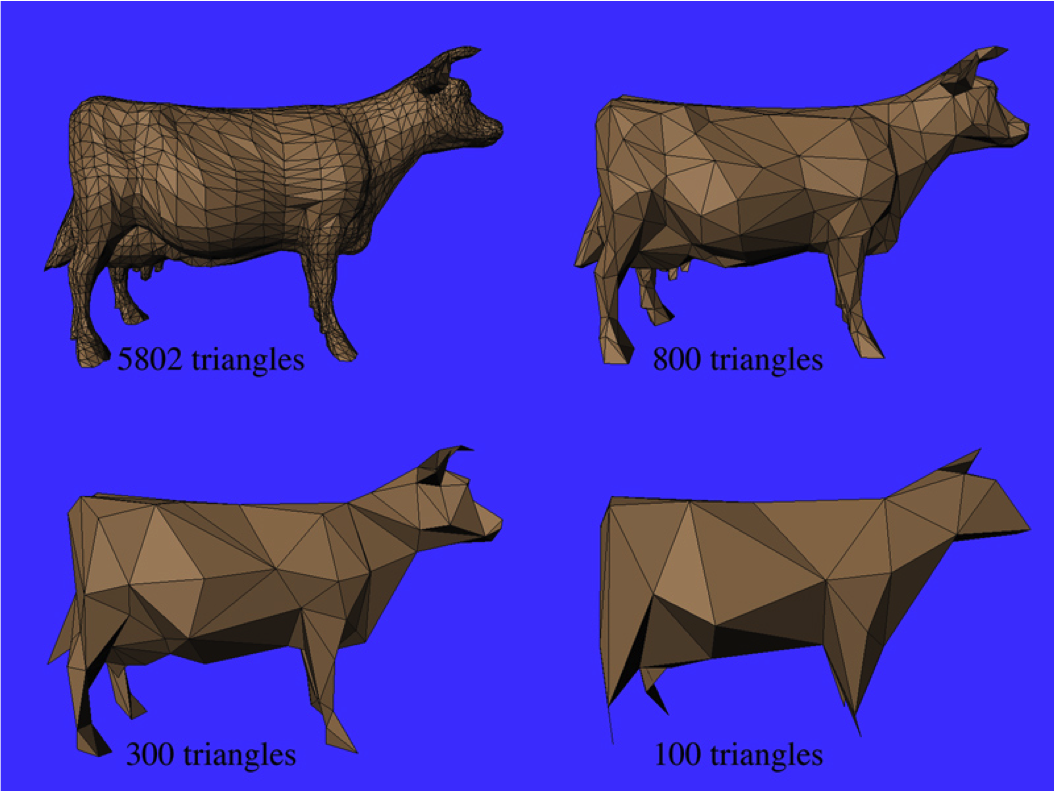
\includegraphics[height=.8\textheight]{figs/triangles}
\end{center}
\end{frame}

\begin{frame}{Surfaces de révolution}
\begin{columns}
\begin{column}{.6\textwidth}
\begin{itemize}
\item Un axe et un profil
\item L'objet peut être décomposé en facettes quadrangulaires
\item Et donc en triangles
\end{itemize}
\end{column}
\begin{column}{.39\textwidth}
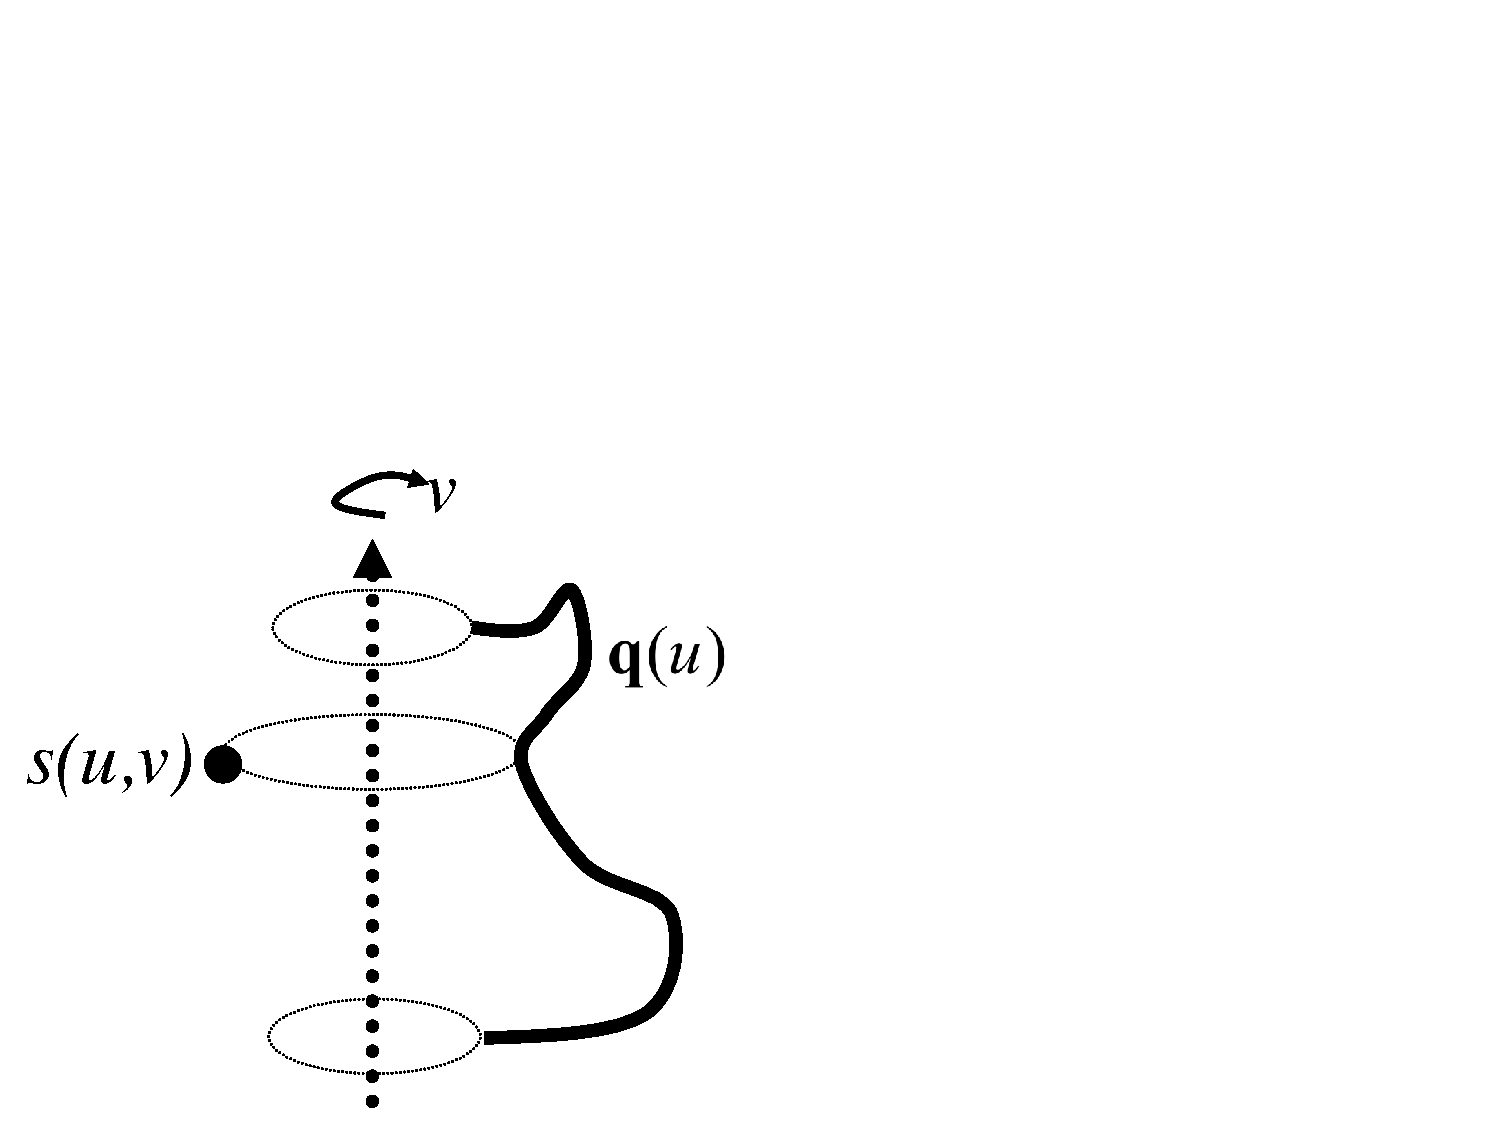
\includegraphics[height=.4\textheight]{figs/rev2.pdf} \\
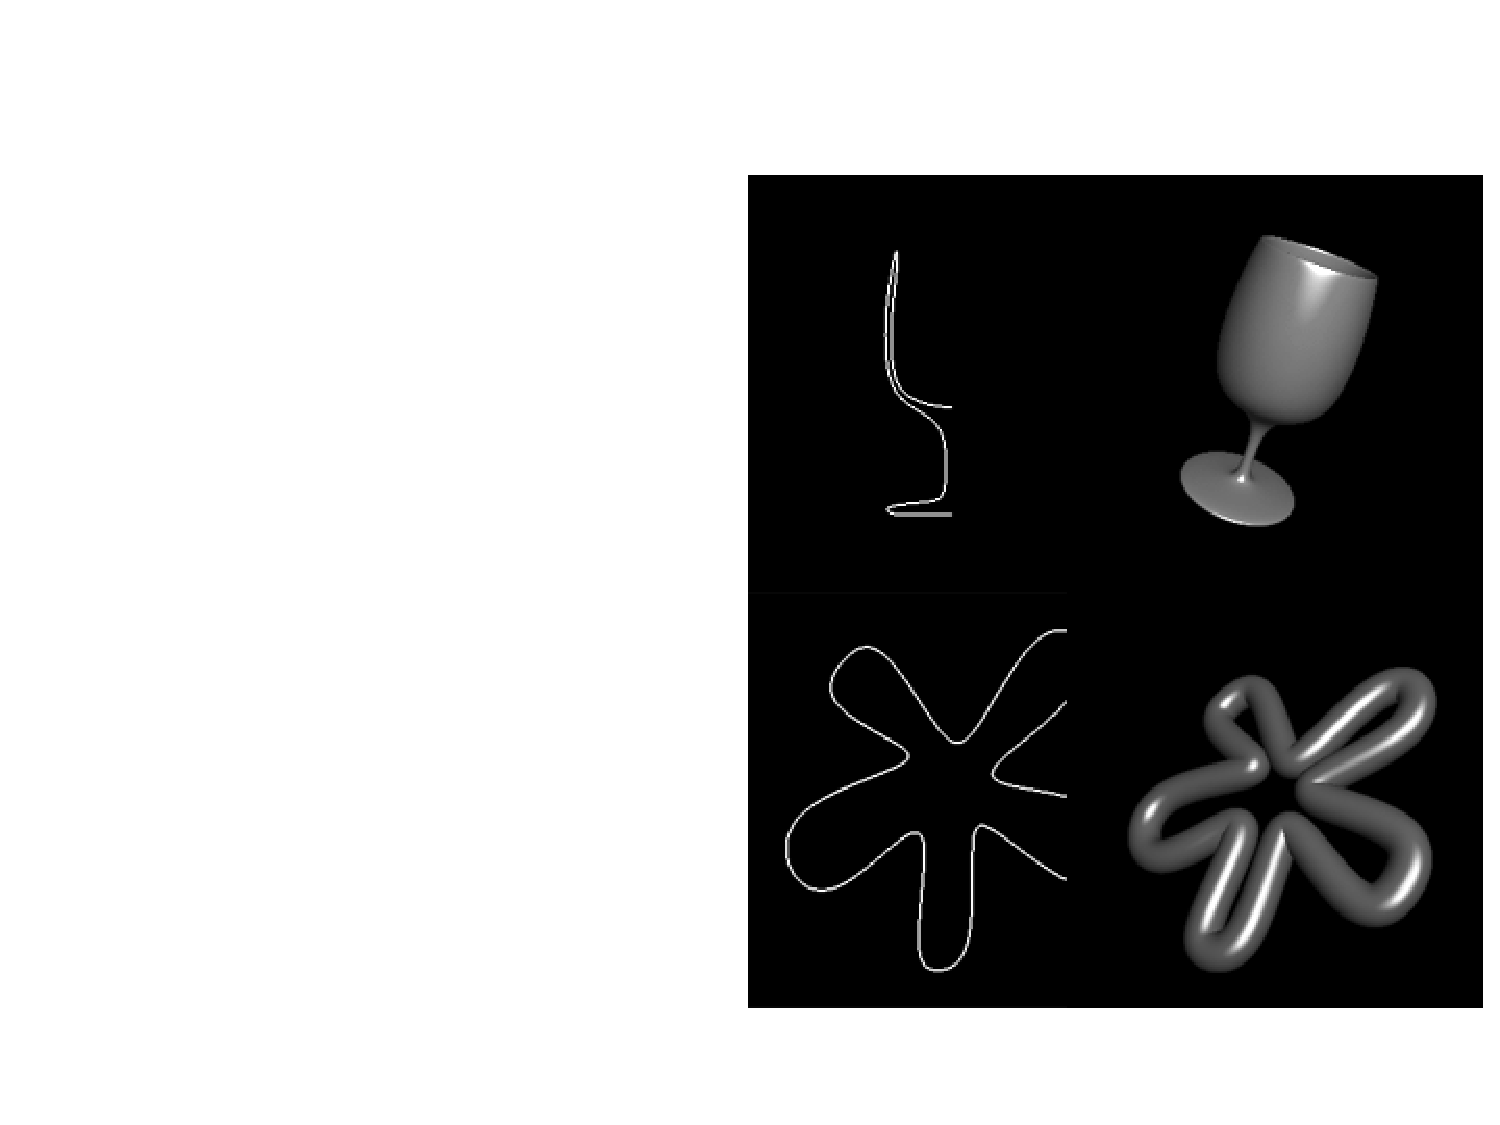
\includegraphics[height=.4\textheight]{figs/rev1.pdf}
\end{column}
\end{columns}
\end{frame}

\begin{frame}{CSG: constructive solid geometry}
\begin{columns}
\begin{column}{.6\textwidth}
\begin{itemize}
\item Combinaison de primitives géométriques
\item Opérateurs ensemblistes
\begin{itemize}
\item Union
\item Intersection
\item Différence
\end{itemize}
\item Très utilisé en CAO
\item Transformable (difficilement) en maillage triangulé
\item Utilisable directement dans certains algorithmes de rendu
\end{itemize}
\end{column}
\begin{column}{.39\textwidth}
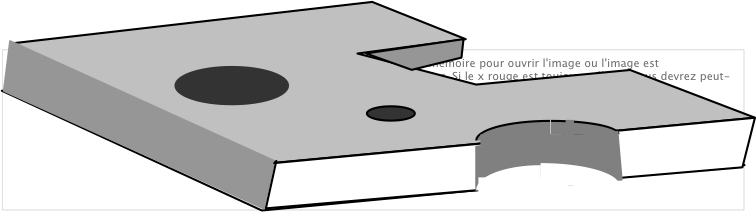
\includegraphics[width=.8\textwidth]{figs/csg1.png} \\
\vspace{1cm}
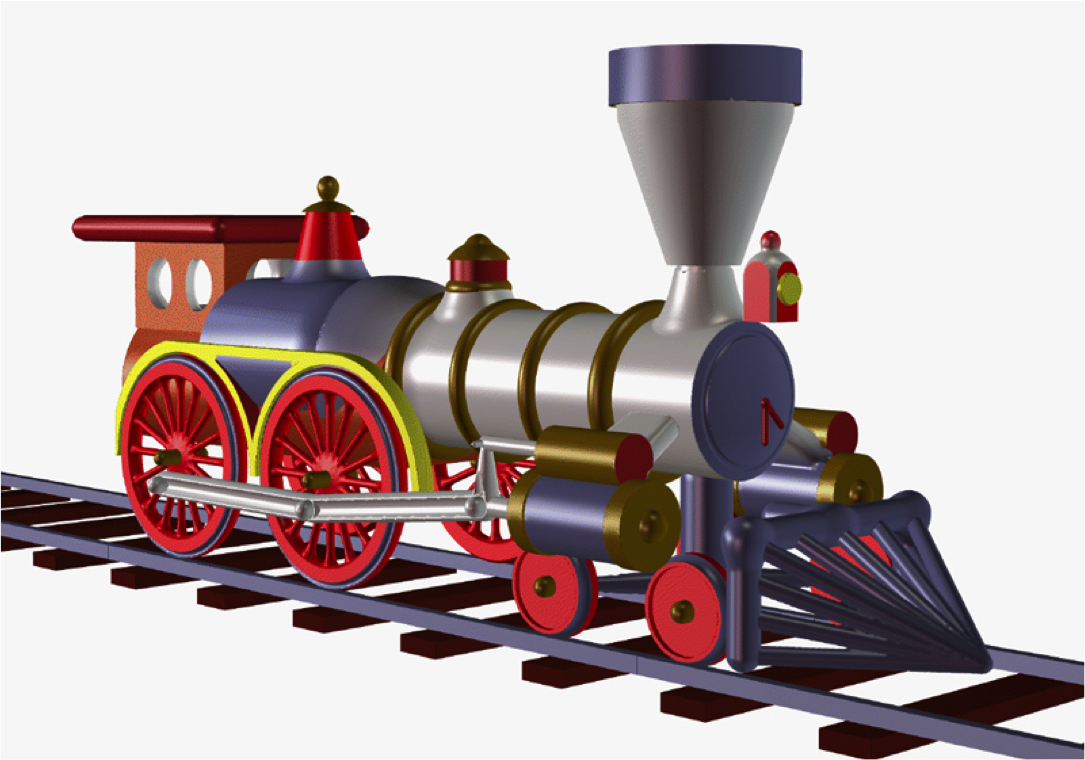
\includegraphics[width=.8\textwidth]{figs/csg2.png}
\end{column}
\end{columns}
\end{frame}

\subsection{Le pipeline graphique}

\begin{frame}{Pipeline graphique}
\begin{itemize}
\item Pipeline graphique : série de transformations géométriques
\end{itemize}
\begin{center}
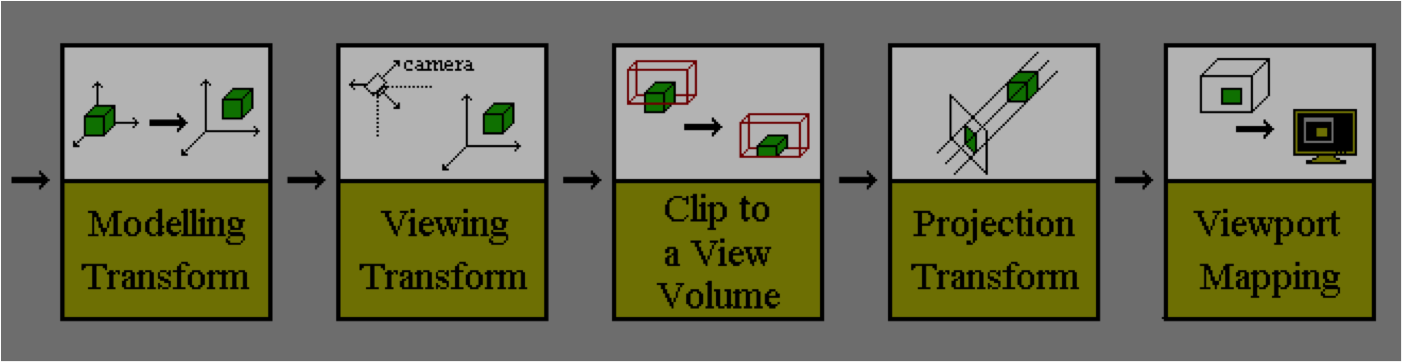
\includegraphics[width=.8\textwidth]{figs/pipeline.png}
\end{center}
\end{frame}

\begin{frame}{Exemple : série de transformations géométriques}
\begin{columns}
\begin{column}{.6\textwidth}
\begin{itemize}
\item<1-3> Objet dans son repère local
\item<2-3> Plusieurs objets
\item<3> Plusieurs objets vus de la caméra
\end{itemize}
\end{column}
\begin{column}{.39\textwidth}
\includegraphics<1>[width=.8\textwidth]{figs/pp1.png}
\includegraphics<2>[width=.8\textwidth]{figs/pp2.png}
\includegraphics<3>[width=.8\textwidth]{figs/pp3.png}

\end{column}
\end{columns}
\end{frame}

\begin{frame}{Types de repère}
\begin{itemize}
\item Repère objet (plusieurs)
\item Repère observateur
\item Repère écran
\begin{itemize}
\item Entre l'observateur et la scène
\end{itemize}
\end{itemize}
\begin{center}
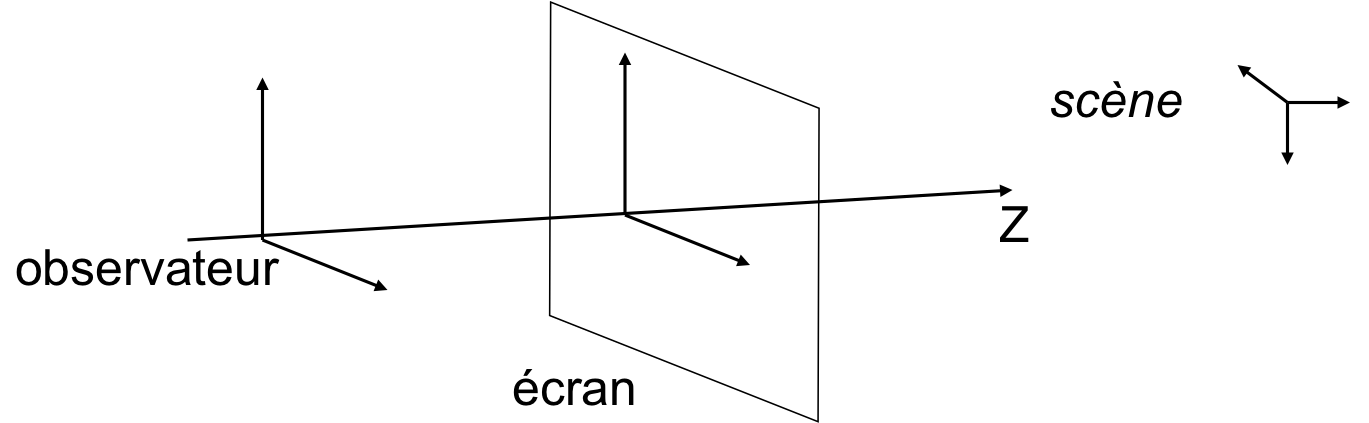
\includegraphics[width=.8\textwidth]{figs/reperes.png}
\end{center}
\end{frame}

\begin{frame}{Modèles hiérarchiques}
\begin{itemize}
\item Les triangles (ainsi que les autres modèles vus précédemment) sont les blocs servant à construire des objets réels plus complexes
\item Les modèles hiérarchiques servent à créer des objets du monde réel par agrégation de formes primitives en des objets plus complexes
\end{itemize}
\begin{center}
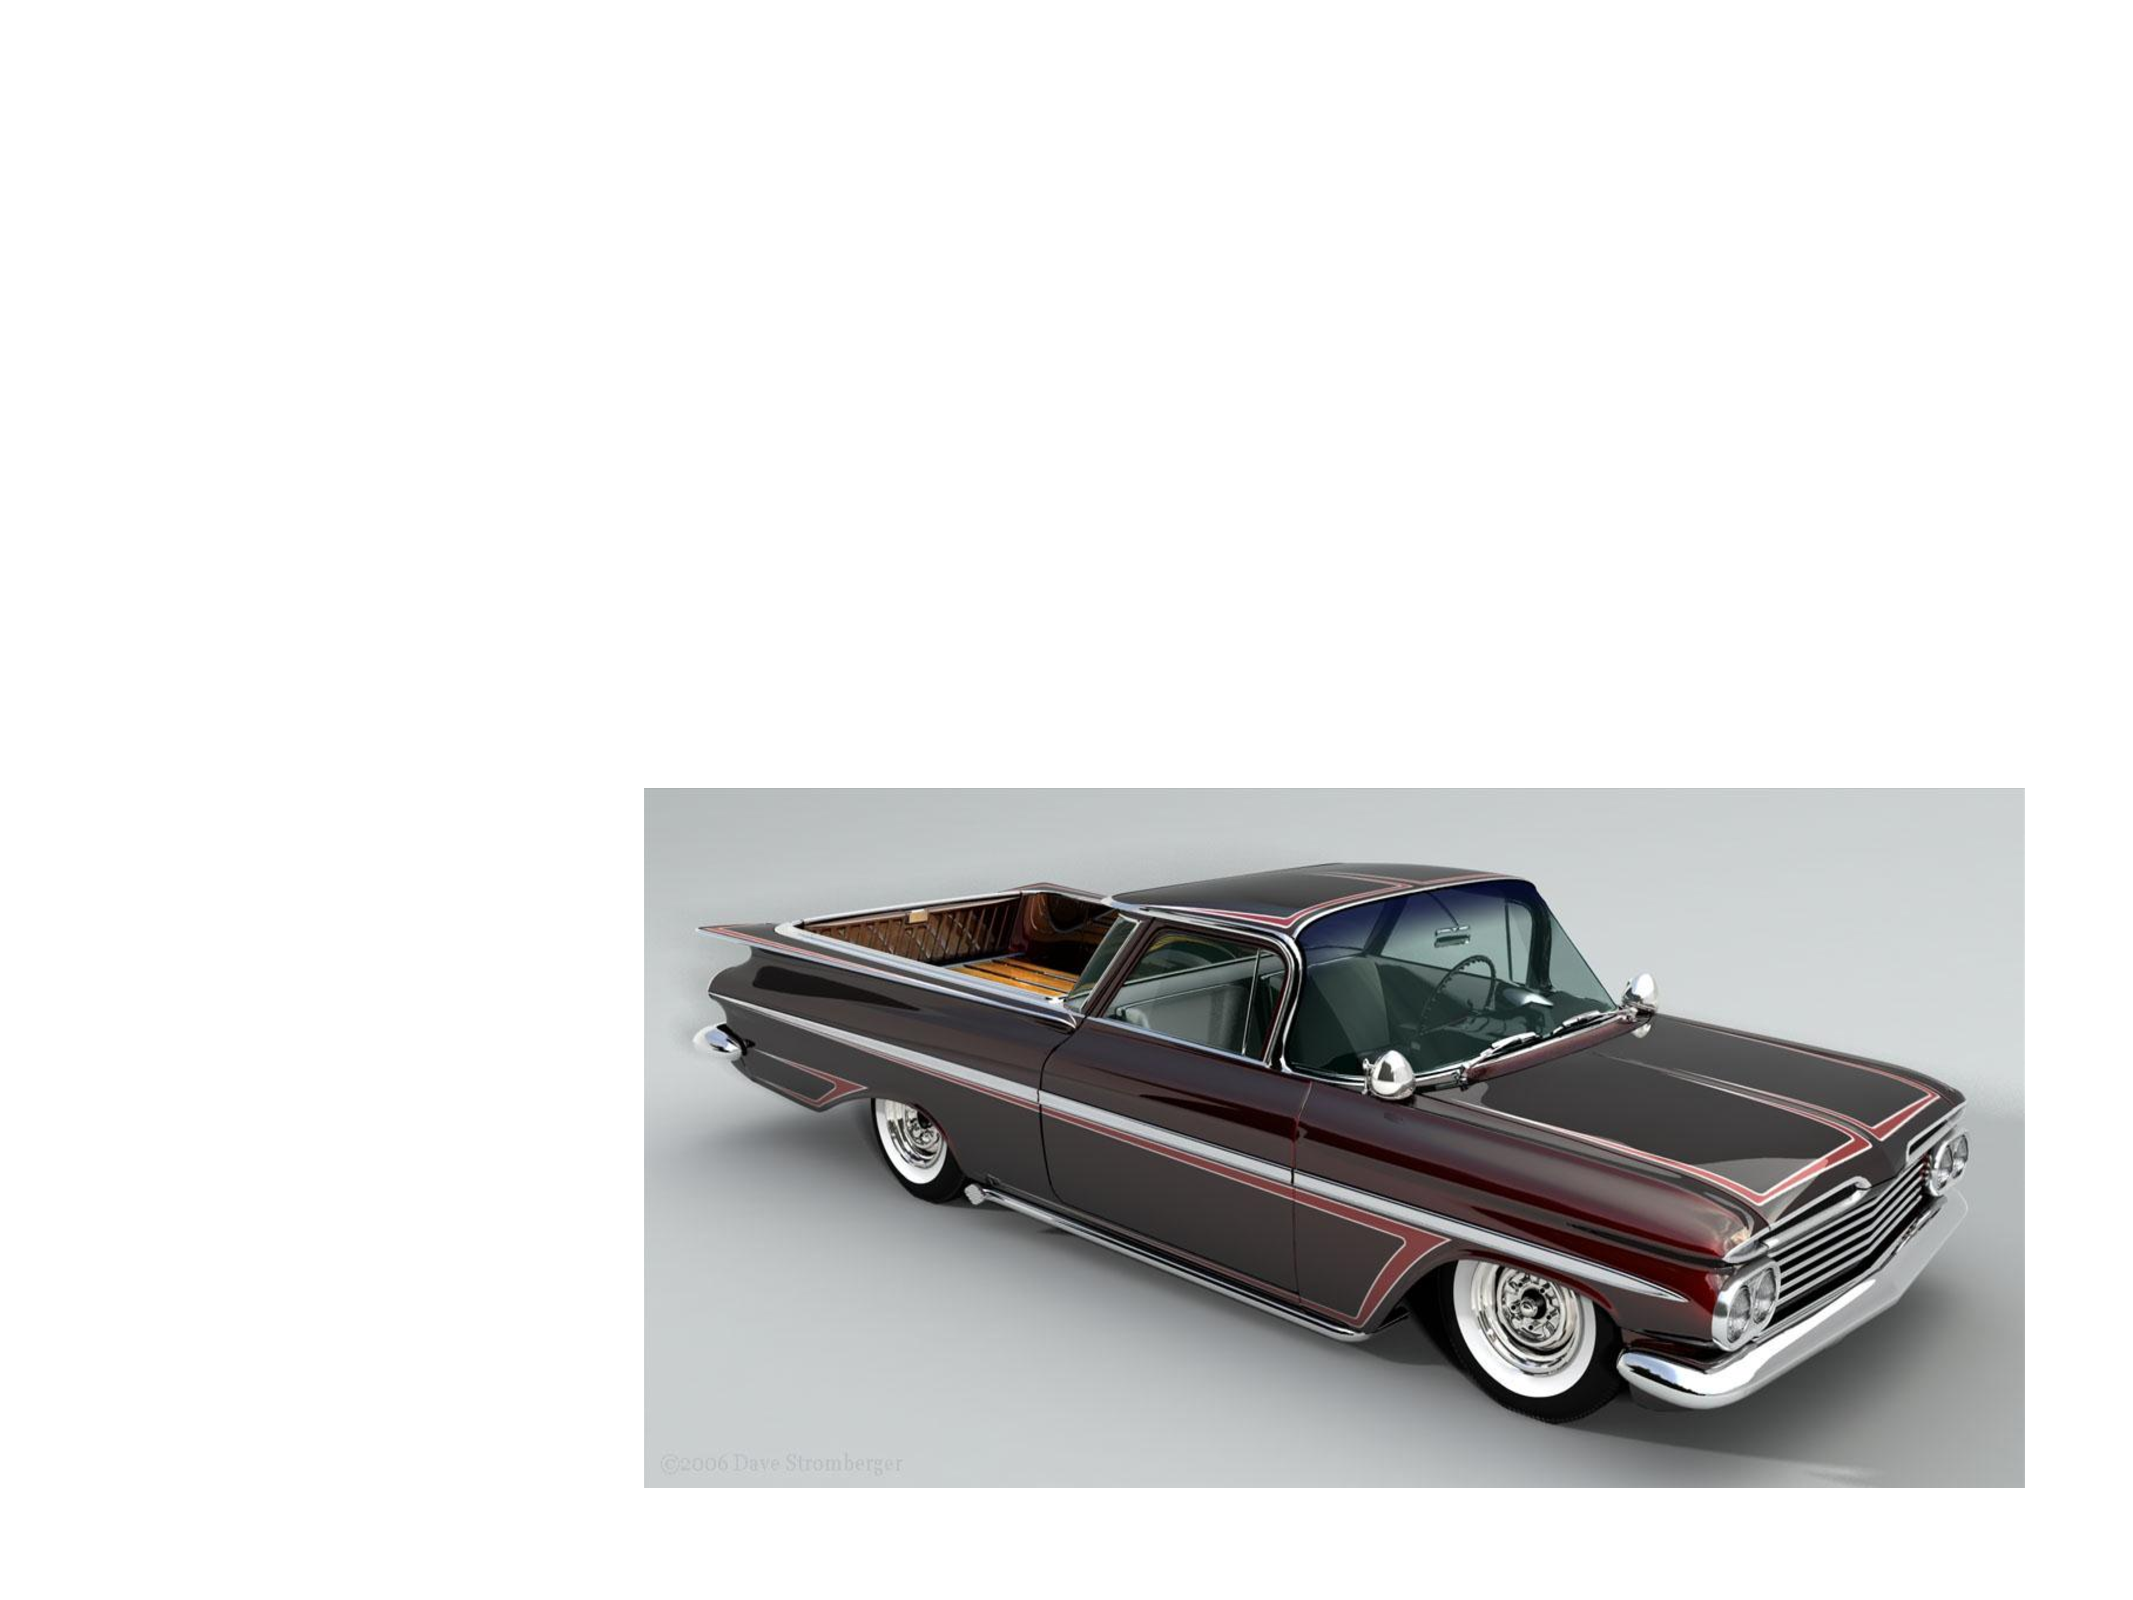
\includegraphics[height=.4\textheight]{figs/car.pdf}
\end{center}

\end{frame}

\begin{frame}{Hiérarchie d'un modèle}
\begin{center}
\includegraphics<1>[height=.8\textheight]{figs/piece1.pdf}
\includegraphics<2>[height=.8\textheight]{figs/piece2.pdf}
\includegraphics<3>[height=.8\textheight]{figs/piece3.pdf}
\includegraphics<4>[height=.8\textheight]{figs/piece4.pdf}
\includegraphics<5>[height=.8\textheight]{figs/piece5.pdf}
\includegraphics<6>[height=.8\textheight]{figs/piece6.pdf}
\end{center}
\end{frame}

\begin{frame}{Vers une notion de <<graphe de scène>>}
\begin{center}
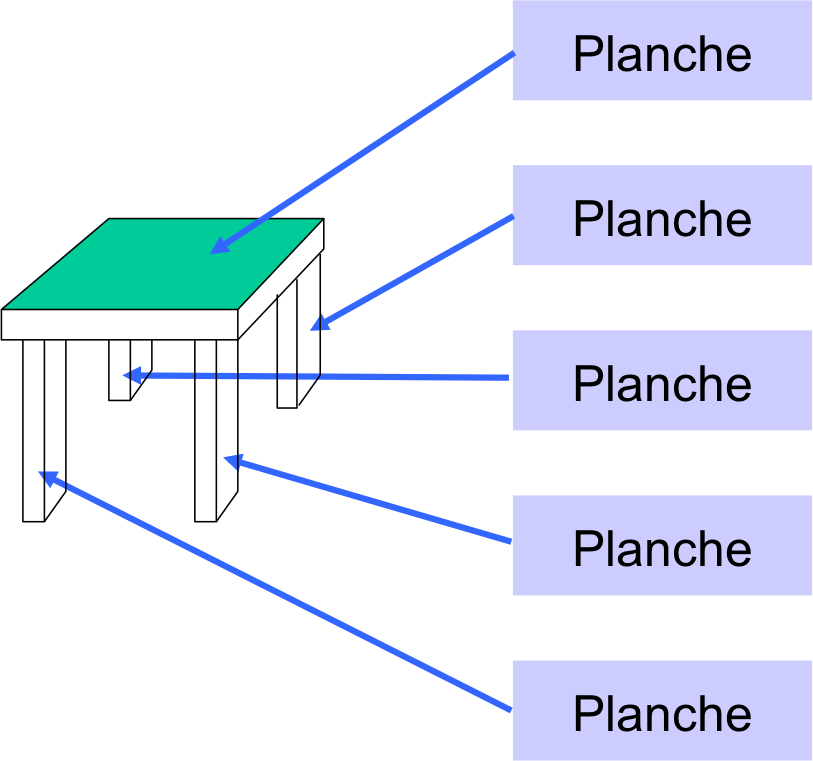
\includegraphics[height=.8\textheight]{figs/table.png}
\end{center}
\end{frame}

\begin{frame}{Vers une notion de <<graphe de scène>>}
\begin{center}
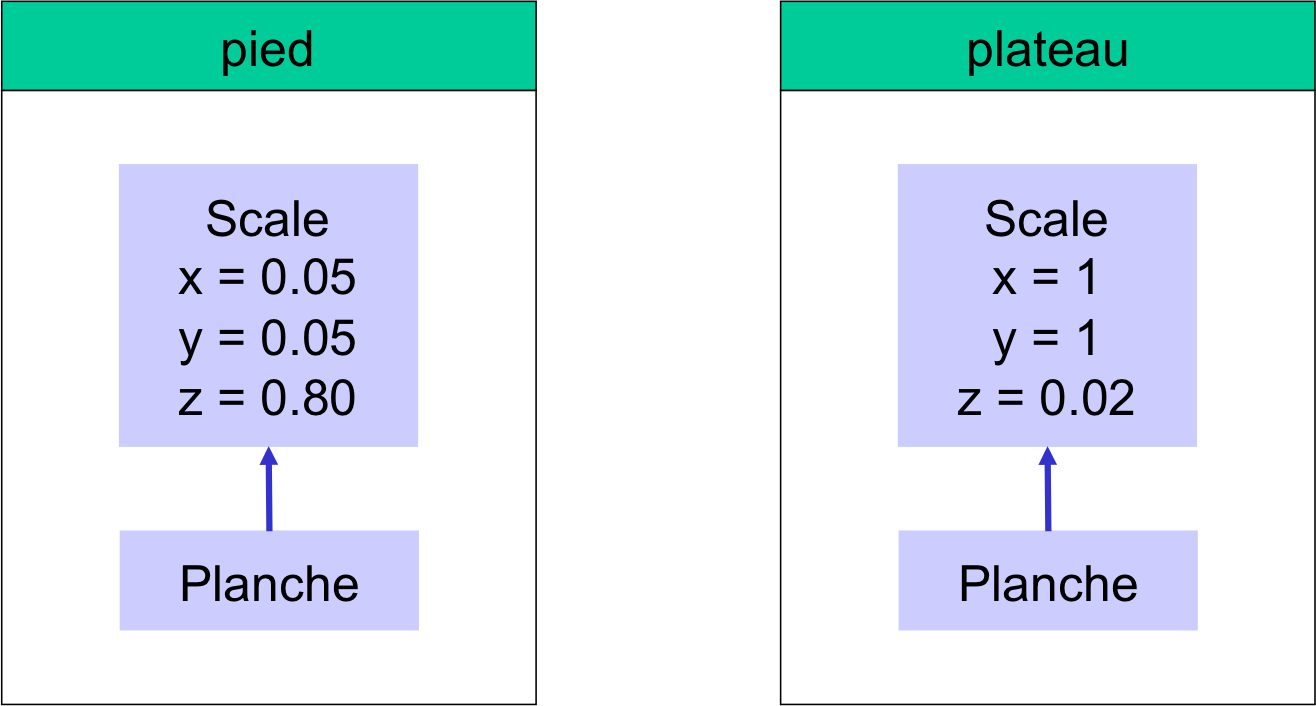
\includegraphics[height=.6\textheight]{figs/table2.png}
\end{center}
\end{frame}

\begin{frame}{Vers une notion de <<graphe de scène>>}
\begin{center}
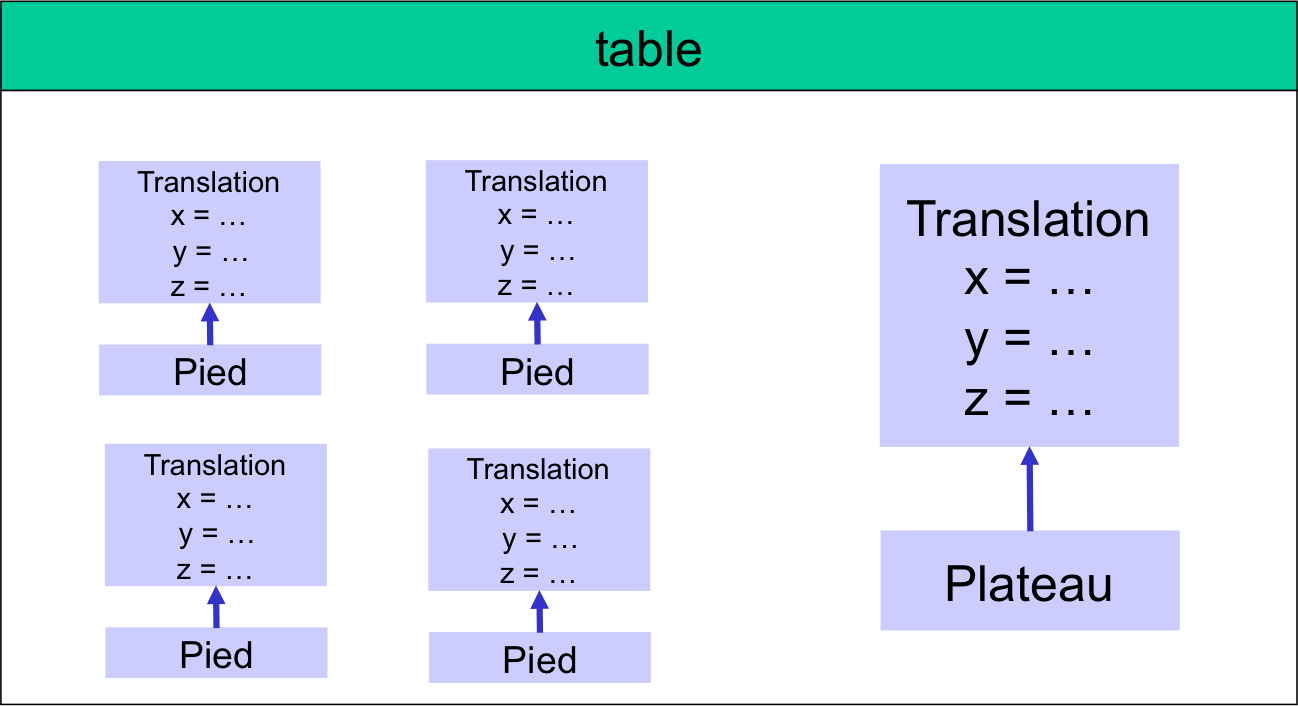
\includegraphics[height=.6\textheight]{figs/table3.png}
\end{center}
\end{frame}

\begin{frame}{Vers une notion de <<graphe de scène>>}
\begin{center}
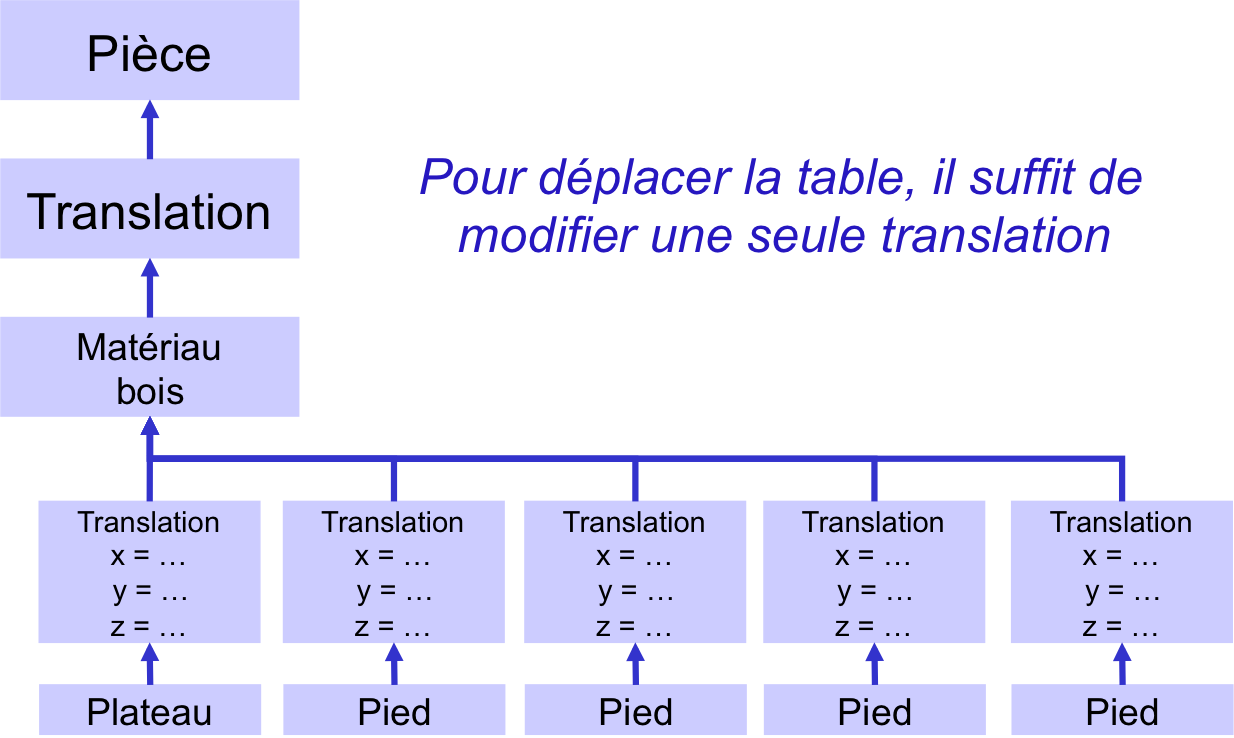
\includegraphics[height=.6\textheight]{figs/table4.png}
\end{center}
\end{frame}

\begin{frame}{Différentes formes de graphes de scène}
\begin{center}
\includegraphics<1>[height=.8\textheight]{figs/sg1.png}
\includegraphics<2>[height=.8\textheight]{figs/sg2.png}
\includegraphics<3>[height=.5\textheight]{figs/sg3.png}
\includegraphics<4>[height=.6\textheight]{figs/sg4.png}
\end{center}
\end{frame}


\begin{frame}{Graphe de scène}
\begin{columns}
\begin{column}{.6\textwidth}
\begin{itemize}
\item Structure de données pratique pour la représentation de scènes
\begin{itemize}
\item Géométrie (dont maillages)
\item Transformations géométriques
\item Matériaux, couleurs
\item Multi-instanciations
\end{itemize}
\item Basé sur un simple arbre hiérarchique
\item Utile pour l'animation et la manipulation
\begin{itemize}
\item Exemple : figure articulée
\end{itemize}
\item Utile pour le rendu
\begin{itemize}
\item Accélération du lancer de rayons
\item Gestion des occlusions
\end{itemize}
\end{itemize}
\end{column}
\begin{column}{.39\textwidth}
\begin{center}
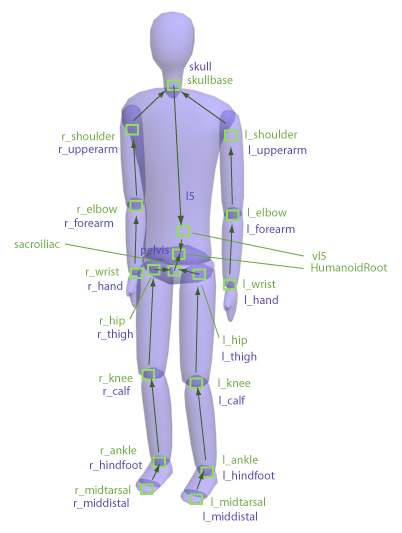
\includegraphics[width=.8\textwidth]{figs/hanim.jpg}
\end{center}
\end{column}
\end{columns}
\end{frame}

\begin{frame}{Modèles hiérarchiques et OpenGL}
\begin{alertblock}{Remarque}
Ou pourquoi il faut éviter de programmer des choses complexes avec OpenGL
\end{alertblock}
\begin{itemize}
\item OpenGL s'apparente à de la programmation procédurale
\begin{itemize}
\item Séquence de dessin des différentes primitives de l'objet
\item Des opérations qui modifient la transformation courante
\begin{itemize}
\item \texttt{glTranslate()}, \texttt{glScale()}...
\end{itemize}
\end{itemize}
\item Les transformations géométriques affectent l'état courant, et donc tout ce qui suit
\item En OpenGL, on va utiliser \texttt{glPushMatrix()} et \texttt{glPopMatrix()} pour enregistrer / récupérer l'état courant
\item Lorsqu'on rencontre un noeud \textit{Transform}
\begin{itemize}
\item \texttt{glPushMatrix()}
\item Application de la transformation géométrique
\item dessin du noeud et de ses sous-noeuds
\item \texttt{glPopMatrix()}
\end{itemize}
\end{itemize}
\end{frame}


\subsection{Coordonnées homogènes}

\begin{frame}{En deux dimensions}
\begin{itemize}
\item 2D : plus facile à représenter mais exactement le même principe
\item Transformation géométrique d'un point $\mathbf{X}=(x,y)$
\begin{eqnarray*}
x' & = & f(x,y) \\
y' & = & g(x,y)
\end{eqnarray*}
\item Comment peut-on représenter les transformations courantes ?
\end{itemize}
\end{frame}

\begin{frame}{Translation}
\begin{columns}
\begin{column}{.6\textwidth}
\begin{itemize}
\item Très simple
\begin{eqnarray*}
x' & = & x + t_x \\
y' & = & y + t_y
\end{eqnarray*}
\item Notation vectorielle
\end{itemize}
\begin{eqnarray}
\mathbf{X'} & = & \mathbf{X} + \mathbf{t}
\end{eqnarray}
\end{column}
\begin{column}{.39\textwidth}
\begin{center}
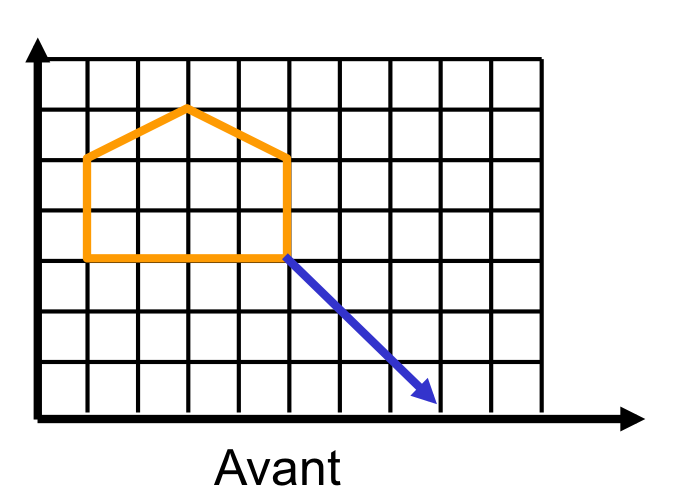
\includegraphics[width=.7\textwidth]{figs/trans2d1.png} \\
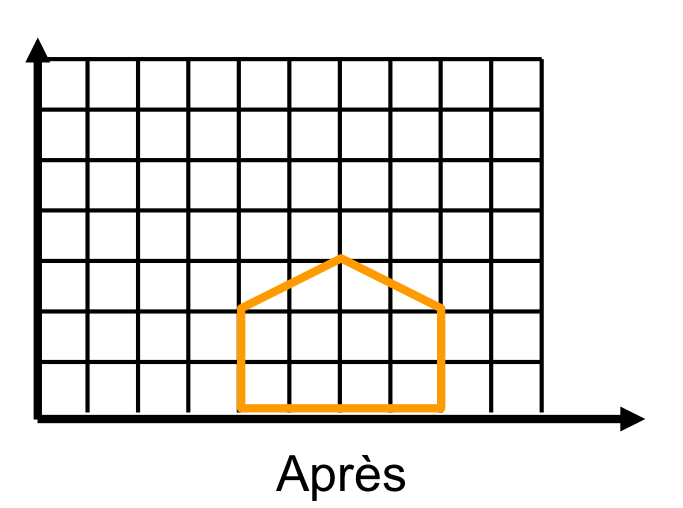
\includegraphics[width=.7\textwidth]{figs/trans2d2.png} \\

\end{center}
\end{column}
\end{columns}
\end{frame}

\begin{frame}{Changement d'échelle}
\begin{columns}
\begin{column}{.6\textwidth}
\begin{itemize}
\item Centré sur l'origine
\item Il suffit d'appliquer une translation préalable
\begin{eqnarray*}
x' & = & x . s_x \\
y' & = & y . s_y
\end{eqnarray*}
\item Notation vectorielle
\end{itemize}
\begin{eqnarray*}
\mathbf{X'} & = & \mathbf{S}\mathbf{X} \\
\mathrm{avec}\  \mathbf{S} & = & \left(
\begin{array}{cc}
s_x & 0 \\
0 & s_y \\
\end{array}
\right)
\end{eqnarray*}
\end{column}
\begin{column}{.39\textwidth}
\begin{center}
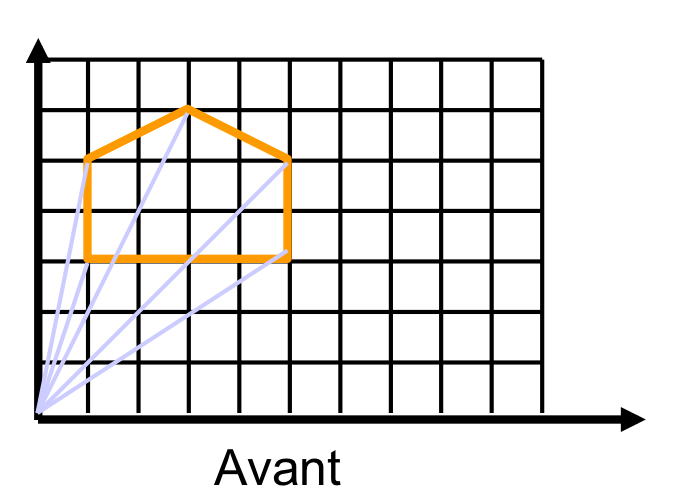
\includegraphics[width=.7\textwidth]{figs/scale1.png} \\
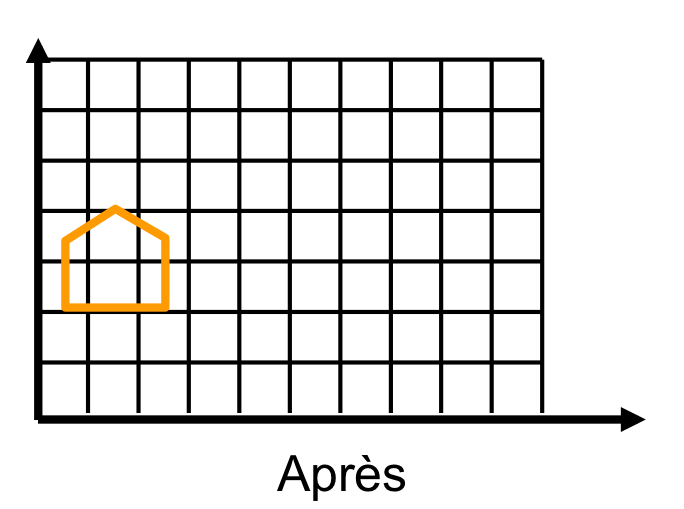
\includegraphics[width=.7\textwidth]{figs/scale2.png} \\

\end{center}
\end{column}
\end{columns}
\end{frame}

\begin{frame}{Rotation, notation unifiée}
\begin{itemize}
\item De façon similaire, on écrit la rotation d'un angle $\theta$ par rapport à l'origine :
\begin{eqnarray*}
\mathbf{X'} & = & \mathbf{R}\mathbf{X} \\
\mathrm{avec}\  \mathbf{R} & = & \left(
\begin{array}{cc}
\cos \theta & -\sin \theta \\
\sin \theta & \cos \theta \\
\end{array}
\right)
\end{eqnarray*}
\item On souhaiterait avoir une notation unifiée
\begin{itemize}
\item Pas un mélange d'additions et de rotations
\item Un seul type d'opérations : bien pour les cartes graphiques
\end{itemize}
\end{itemize}
\end{frame}

\begin{frame}{Coordonnées homogènes}
\begin{itemize}
\item Outil géométrique très puissant
\begin{itemize}
\item Utilisé partout en image (infographie, vision...)
\item Voir géométrie projective
\end{itemize}
\item Consiste à ajouter une $n+1$-ème coordonnée à tout point de dimension $n$
\item Par exemple, en 2D
$$ \mathbf{\overline{X}} = \left( \begin{array}{c} x \\ y \\ w
\end{array}\right), w \neq 0 $$
\item Deux points sont égaux ssi $x'/w'=x/w$ et $y'/w'=y/w$
\item $w=0$ utile pour représenter les points à l'infini (points de fuite, projections...)
\end{itemize}
\end{frame}

\begin{frame}{Translation en coordonnées homogènes}
\begin{center}
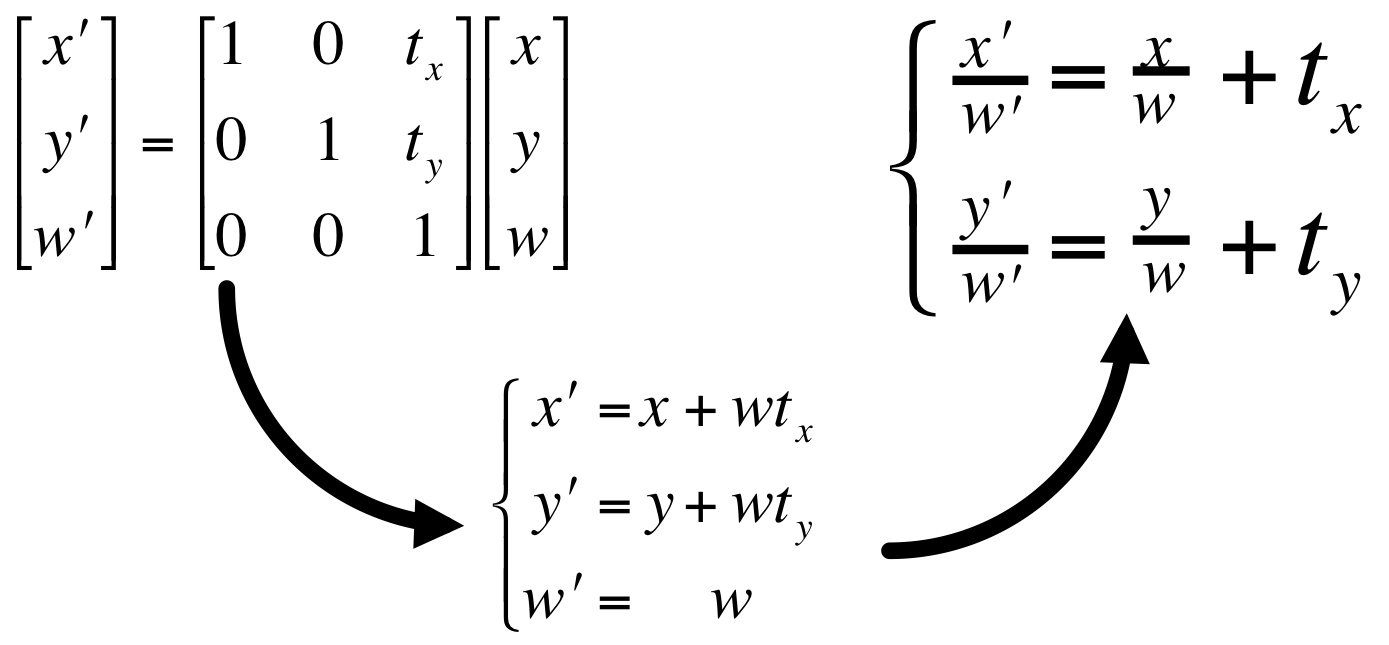
\includegraphics[width=.8\textwidth]{figs/transh.png}
\end{center}
\end{frame}

\begin{frame}{Changement d'échelle en coordonnées homogènes}
\begin{center}
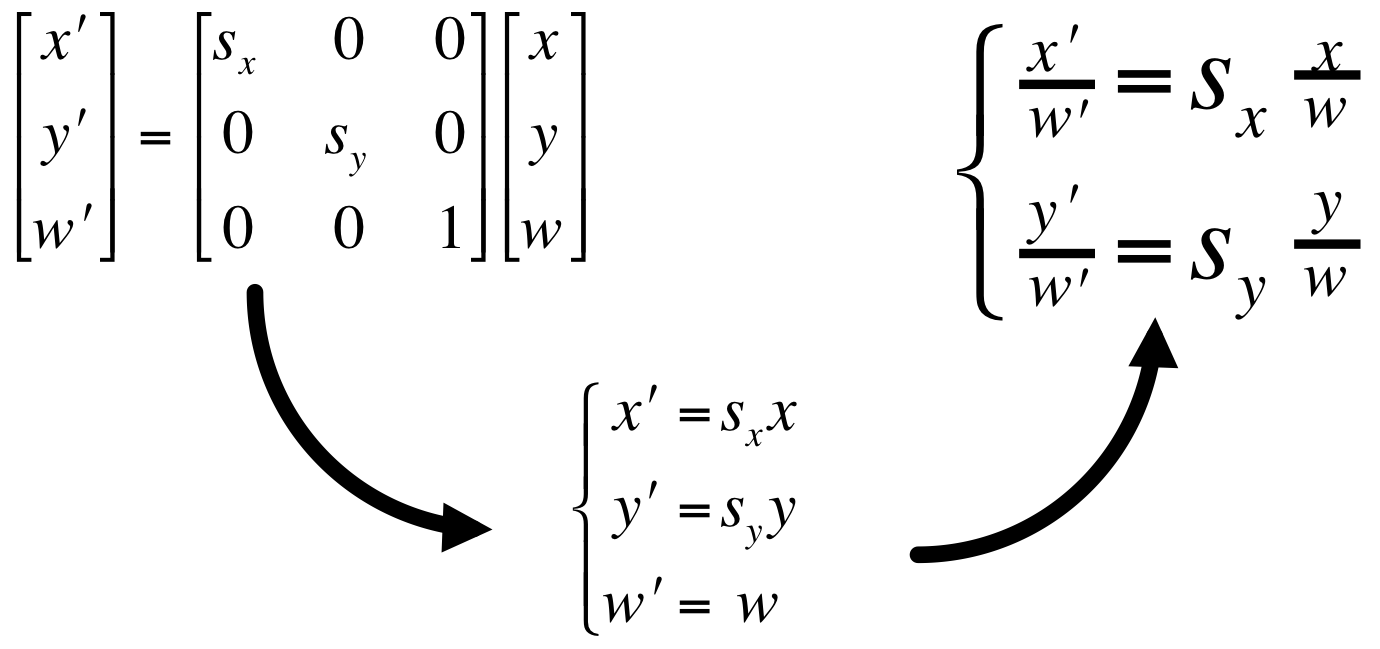
\includegraphics[width=.8\textwidth]{figs/scaleh.png}
\end{center}
\end{frame}

\begin{frame}{Rotation en coordonnées homogènes}
\begin{center}
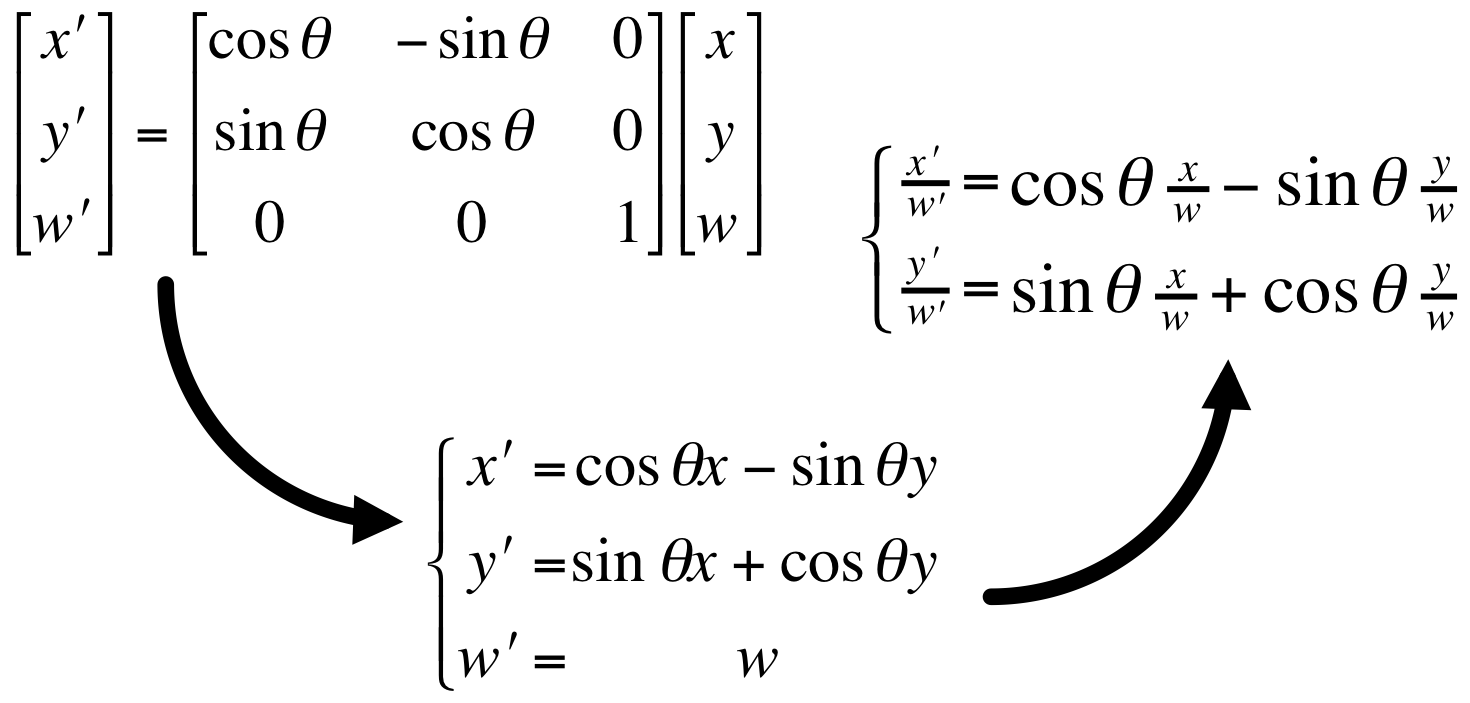
\includegraphics[width=.8\textwidth]{figs/roth.png}
\end{center}
\end{frame}

\begin{frame}{Composition de transformations}
\begin{itemize}
\item Toutes les transformations homogènes s'expriment sous forme de matrices
\item Il suffit de multiplier les matrices !
\item En se rappelant que la multiplication de matrices n'est pas commutative
\item Exemple : rotation autour d'un point $\mathbf{Q}$
\begin{itemize}
\item Translater $\mathbf{Q}$ à l'origine
\item Effectuer la rotation
\item Translater en retour vers $\mathbf{Q}$
$$
\mathbf{Q'} = -\mathbf{T_Q R_{\theta} T_Q P}
$$
\end{itemize}
\end{itemize}
\end{frame}


\begin{frame}{Translations en 3D}
\begin{center}
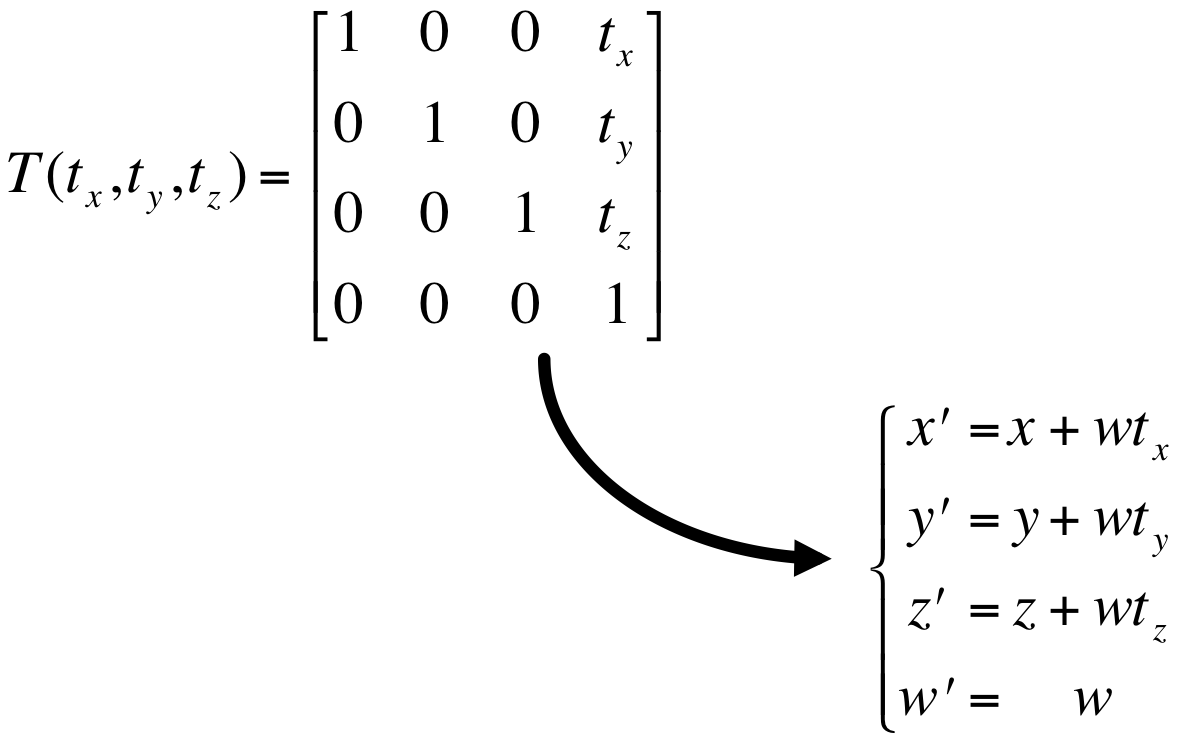
\includegraphics[width=.8\textwidth]{figs/transh3.png}
\end{center}
\end{frame}

\begin{frame}{Changements d'échelle en 3D}
\begin{center}
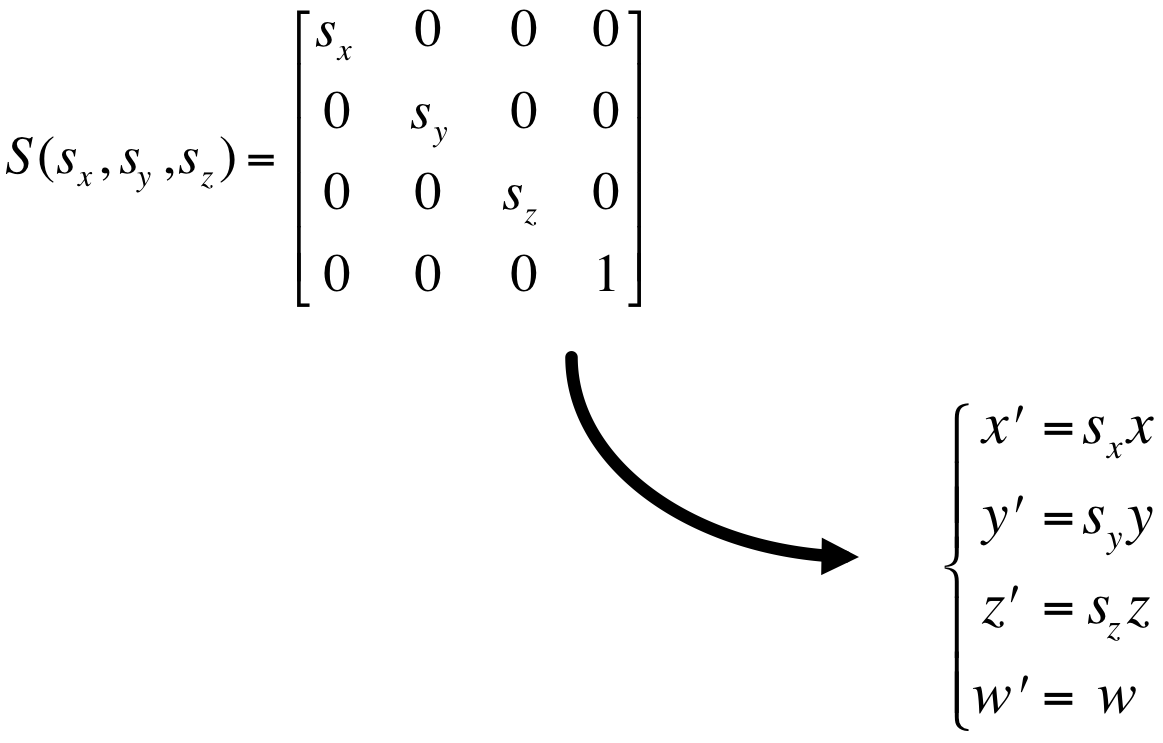
\includegraphics[width=.8\textwidth]{figs/scaleh3.png}
\end{center}
\end{frame}

\begin{frame}{Rotations en 3D}
\begin{itemize}
\item Rotation en 3D : définie par un axe et un angle
\item La matrice peut être construite à partir de l'axe et de l'angle
\item Expression directe avec un peu de calcul vectoriel
\begin{itemize}
\item Outil pratique : les quaternions
\end{itemize}
\item OpenGL peut le faire pour vous
\begin{itemize}
\item \texttt{glRotatef(angle,x,y,z)}
\end{itemize}
\end{itemize}
\end{frame}

\begin{frame}{Bilan : transformations 3D}
\begin{itemize}
\item Toutes les transformations 3D s'expriment sous forme de matrice homogène
\begin{itemize}
\item translations, rotations, changement d'échelle
\item et même d'autres que nous verrons plus tard
\end{itemize}
\item et donc leur combinaison comme une multiplication de matrices homogènes
\item La bibliothèque graphique fournit les fonctions adéquates
\begin{itemize}
\item \texttt{glTranslatef(x,y,z)}
\item \texttt{glRotatef(angle,x,y,z)}
\item \texttt{glScalef(x,y,z)}
\end{itemize}
\end{itemize}
\end{frame}

\begin{frame}{Composition de transformations avec OpenGL}
\begin{itemize}
\item Outils pour construire ses transformations
\begin{itemize}
\item \texttt{glLoadIdentity()}
\item \texttt{glLoadMatrixf()}
\item \texttt{glMultMatrixf()}
\end{itemize}
\item Gestion de la hiérarchie
\begin{itemize}
\item \texttt{glPushMatrix()}
\item \texttt{glPopMatrix()}
\end{itemize}
\item Mais aussi des fonctions de plus haut niveau !
\begin{itemize}
\item \texttt{gluLookAt(Eyex, Eyey, Eyez,Centerx, Centery, Centerz, upx, upy, upz)}
\item \texttt{gluPerspective( fovy, aspect, zNear, zFar )}
\end{itemize}
\end{itemize}
\end{frame}

\subsection{Projections}

\begin{frame}{Caméra virtuelle}
\begin{center}
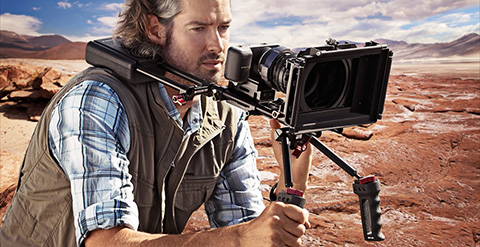
\includegraphics[width=3cm]{figs/camerar.jpg}
\end{center}
\begin{itemize}
\item Métaphore de la caméra
\begin{itemize}
\item Définir une caméra virtuelle qui va filmer la scène (virtuelle)
\item Restitution sur un moniteur 2D
\end{itemize}
\item Il faut
\begin{itemize}
\item Définir les caractéristiques de la caméra
\item Placer et orienter la caméra
\item Prendre les images et les afficher
\end{itemize}
\end{itemize}
\end{frame}

\begin{frame}{Différentes projections}
\begin{center}
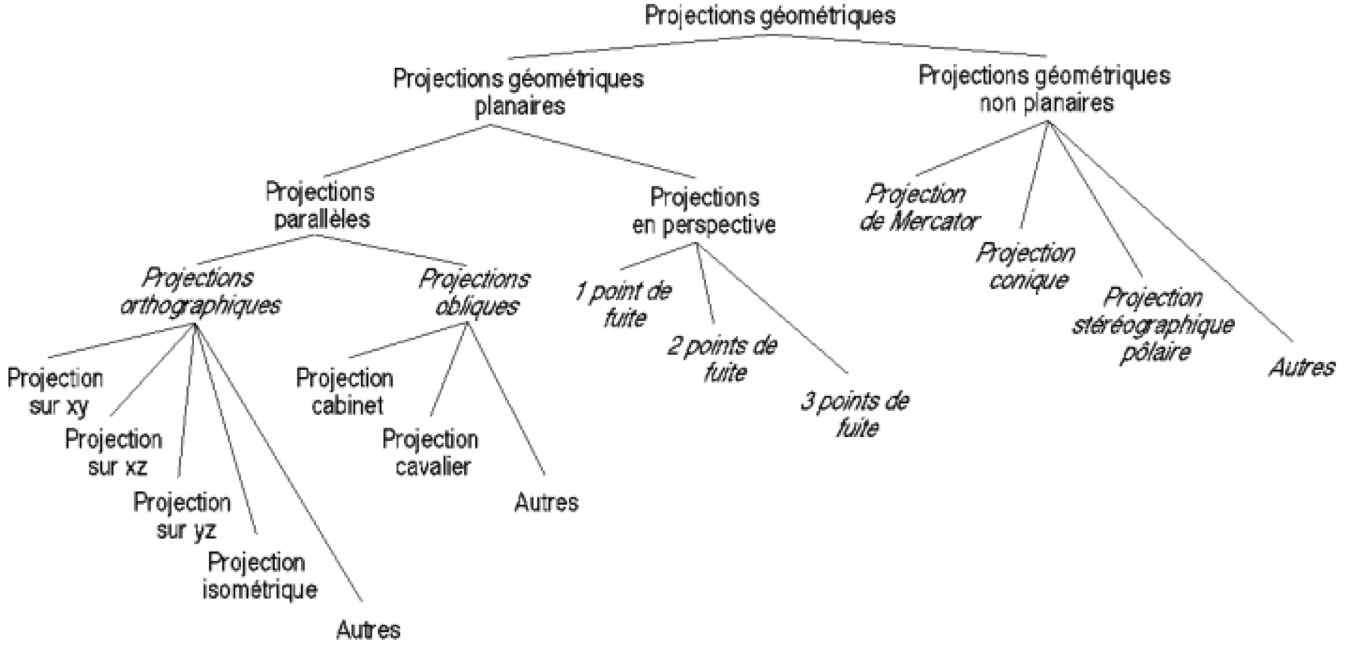
\includegraphics[width=.8\textwidth]{figs/projections.png}
\end{center}
\end{frame}

\begin{frame}{Quelle projection ?}
\begin{center}
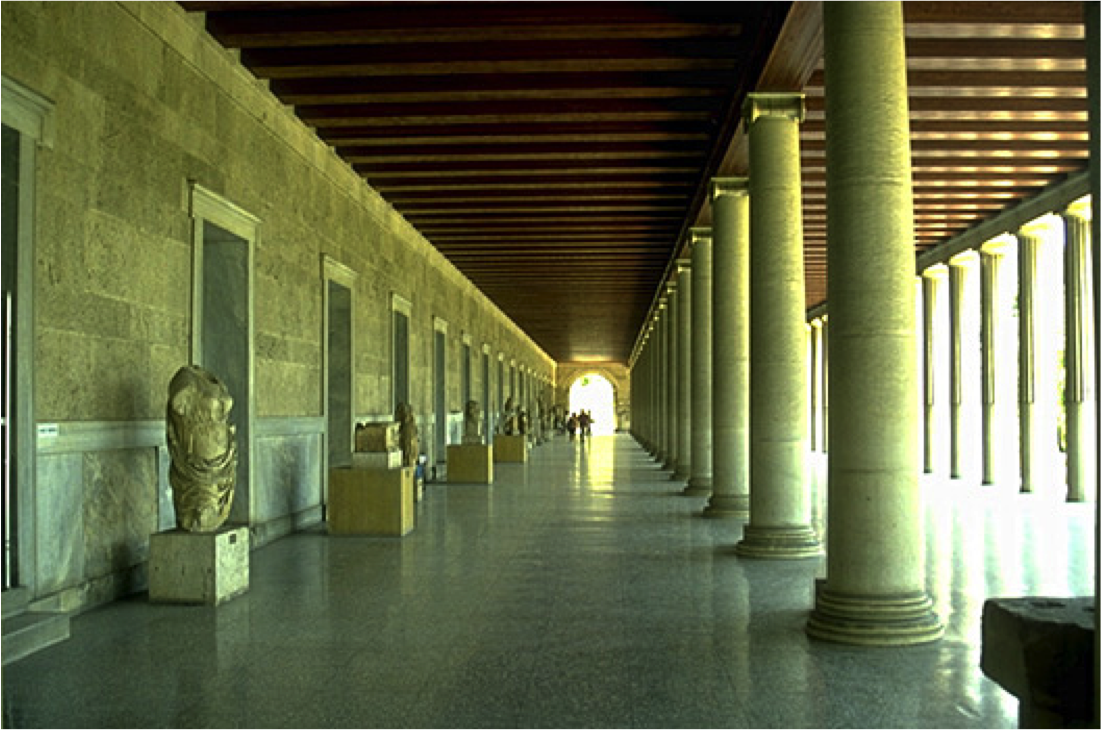
\includegraphics[width=.8\textwidth]{figs/athenes.png}
\end{center}
\end{frame}

\begin{frame}{Projection parallèle vs. perspective}
\begin{center}
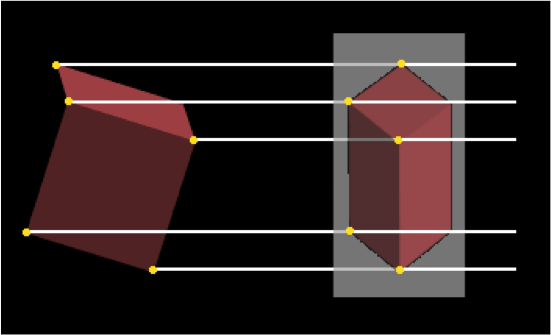
\includegraphics[height=3.7cm]{figs/projpar.png} \\
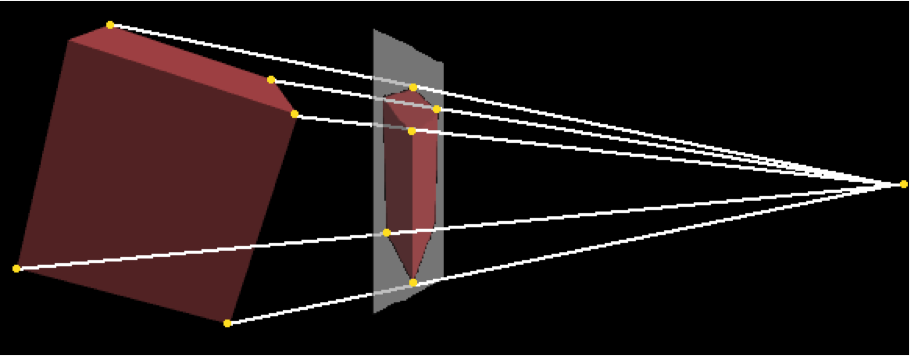
\includegraphics[height=3.7cm]{figs/projpersp.png} \\

\end{center}
\end{frame}

\begin{frame}{Projection parallèle vs. perspective : résultat}
\begin{center}
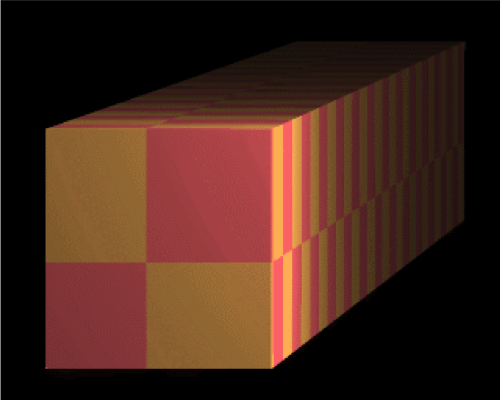
\includegraphics[height=3.7cm]{figs/projparr.png} \hspace{1cm}
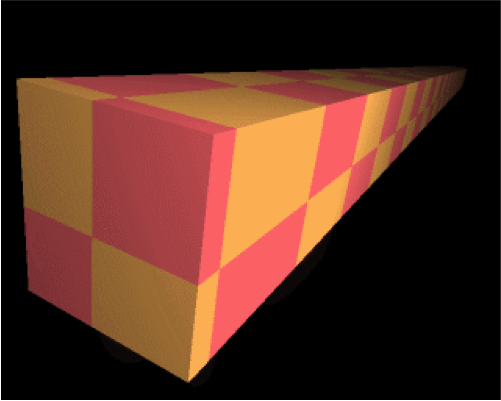
\includegraphics[height=3.7cm]{figs/projpersp1.png} \\

\end{center}
\begin{itemize}
\item L'\oe il humain utilise une projection centrale (perspective), tout comme une caméra
\end{itemize}
\end{frame}

\begin{frame}{Projection perspective simple}
\begin{center}
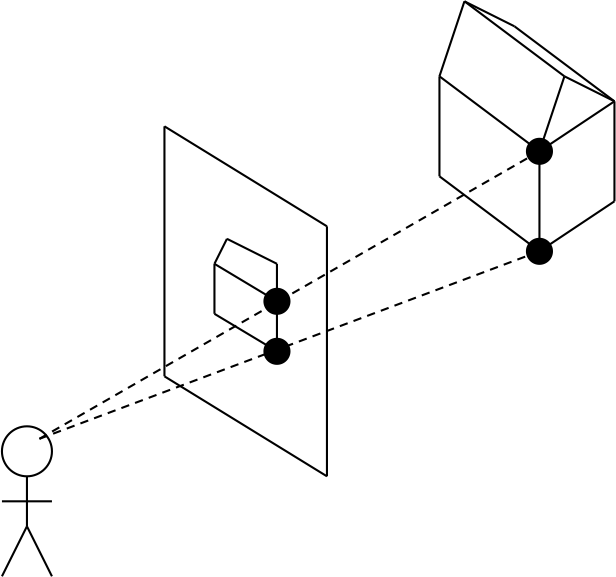
\includegraphics[height=.6\textheight]{figs/persp1.png}
\end{center}
\end{frame}

\begin{frame}{Projection perspective simple}
\begin{itemize}
\item Caméra dans l'axe des $z$
\item Point focal à l'origine
\item Plan image sur le plan XY à une distance $f$
\end{itemize}
\begin{center}
\includegraphics[height=.6\textheight]{figs/persp2.png}
\end{center}
\end{frame}

\begin{frame}{Calcul de la projection}
\begin{eqnarray*}
z' & = & f \\
y'/z' & = & y/z \\
\end{eqnarray*}
\begin{center}
\includegraphics[height=.4\textheight]{figs/persp3.png}
\end{center}
\begin{itemize}
\item Le point $(x,y,z)^t$ se projette sur $\left( (f/z)x,(f/z)y,f \right)^t$
\end{itemize}
\end{frame}

\begin{frame}{Matrice homogène}
\begin{itemize}
\item Projection sur le plan $z=0$ avec le centre de projection placé à $z=-f$

$$
\left(
\begin{array}{cccc}
1 & 0 & 0 & 0 \\
0 & 1 & 0 & 0 \\
0 & 0 & 1 & 0 \\
0 & 0 & \frac{1}{d} & 1
\end{array}
\right)
$$
\item Utilisation de la quatrième coordonnée pour le rétrécissement
\end{itemize}
\end{frame}

\subsection{Autres transformations géométriques}

\begin{frame}{Pyramide de vue (2D)}
\begin{center}
\includegraphics[height=.6\textheight]{figs/frustum2d.pdf}
\end{center}
\end{frame}


\begin{frame}{Clipping}
\begin{columns}
\begin{column}{.6\textwidth}
\begin{itemize}
\item Éliminer les portions des objets qui sont en dehors de la pyramide de vue
\begin{itemize}
\item délimitée par les limites du plan image projeté en 3D et des \textit{near} et \textit{far} plane
\end{itemize}
\item Pourquoi faire ?
\begin{itemize}
\item Ne pas dessiner derrière l'\oe il
\item Limiter la quantité de choses dessinées
\end{itemize}
\item Encore des matrices homogènes !
\end{itemize}
\end{column}
\begin{column}{.39\textwidth}
\begin{center}
\includegraphics[height=.4\textheight]{figs/frustum3d.pdf}
\end{center}
\end{column}
\end{columns}
\end{frame}

\begin{frame}{Backface culling}
\begin{itemize}
\item Élimination des faces vues par l'arrière
\begin{itemize}
\item valable pour les solides non transparents
\end{itemize}
\item Simple produit scalaire entre la normale à une face et le vecteur reliant l'\oe il à cette face
\end{itemize}
\begin{center}
\includegraphics[height=.5\textheight]{figs/bfc.png}
\end{center}
\end{frame}


\section{Couleurs et éclairage}

\begin{frame}{Couleurs et éclairage}
\begin{center}
\includegraphics[height=.6\textheight]{figs/Colored_pencils_chevre.jpg}
\end{center}
\end{frame}

\begin{frame}{Lumière}
\begin{center}
\includegraphics[height=.6\textheight]{figs/prisme.jpg}
\end{center}
\end{frame}

\begin{frame}{Lumière : définition physique}
\begin{columns}
\begin{column}{.6\textwidth}
\begin{itemize}
\item La lumière est caractérisée par son spectre d'absorption
\begin{itemize}
\item La quantité d'énergie pour chaque longueur d'onde
\item Lumière visible : de 380 à 720nm (à peu près)
\begin{itemize}
\item en dessous de 380nm : ultra-violet
\item au dessus de 720nm : infrarouge
\end{itemize}
\end{itemize}
\end{itemize}
\end{column}
\begin{column}{.39\textwidth}
\includegraphics[width=.8\textwidth]{figs/spectre.pdf} \\
\vspace{1cm}
\includegraphics[width=.8\textwidth]{figs/lumsp.png} \\

\end{column}
\end{columns}
\end{frame}

\begin{frame}{Interaction lumière-matière}
\begin{center}
\includegraphics[height=.3\textheight]{figs/lumillum.pdf}
{\Huge .*}
\includegraphics[height=.3\textheight]{figs/lumref.pdf}
{\Huge =}
\includegraphics[height=.3\textheight]{figs/lumsig.pdf}

\end{center}
\begin{itemize}
\item La lumière provient :
\begin{itemize}
\item des sources lumineuses
\item de la réflectance des objets
\end{itemize}
\end{itemize}
\end{frame}

\begin{frame}{Lumière : autre définition}
\begin{itemize}
\item Définition basée sur le vocabulaire usuel de la peinture
\item Utilisant le mélange des couleurs
\end{itemize}
\begin{center}
\includegraphics[height=.6\textheight]{figs/lump.png}
\end{center}
\end{frame}

\begin{frame}{Définition spectrale simplifiée}
\begin{center}
\includegraphics[height=.75\textheight]{figs/lumsimpl.png}
\end{center}
\end{frame}

\begin{frame}{De la lumière à la couleur}

\begin{center}
\includegraphics<1>[width=.8\textwidth]{figs/color1.pdf}
\includegraphics<2>[width=.8\textwidth]{figs/color2.pdf}
\includegraphics<3>[width=.8\textwidth]{figs/color3.pdf}

\end{center}
\begin{itemize}
\item On abordera le système visuel humain dans le cours FONRV
\end{itemize}
\end{frame}

\begin{frame}{Réponse des cônes}
\begin{center}
\includegraphics<1>[height=.8\textheight]{figs/cone.pdf}
\includegraphics<2>[height=.8\textheight]{figs/conecomplet.pdf}
\end{center}
\end{frame}

\begin{frame}{Un cône ne perçoit pas vraiment les couleurs !}
\begin{itemize}
\item Longueur d'onde différente, intensité différente
\item Même réponse
\item<2> Mais réponse différence pour les différents types de cônes
\end{itemize}
\begin{center}
\includegraphics<1>[height=.6\textheight]{figs/conecl.pdf}
\includegraphics<2>[height=.6\textheight]{figs/conecl2.pdf}
\end{center}

\end{frame}

\begin{frame}{Théorie tri-chromatique de von Helmholtz, 1859}
\begin{itemize}
\item Les couleurs sont définis comme des ratios de réponses entre les différents types de cônes
\end{itemize}
\begin{center}
\includegraphics[height=.7\textheight]{figs/couleurs}
\end{center}
\end{frame}

\subsection{Représentation des couleurs}

\begin{frame}{Représentation des couleurs}
\begin{itemize}
\item La représentation spectrale est trop riche
\begin{itemize}
\item Par rapport à la vision humaine
\item En coût mémoire (et de calcul)
\end{itemize}
\item La vision humaine n'a que 3 fonctions de base
\item On doit pouvoir en tirer une représentation compacte
\begin{itemize}
\item A partir de couleurs primaires
\end{itemize}
\end{itemize}
\end{frame}

\begin{frame}{Lois de Grassmman}
\begin{enumerate}
\item toute couleur peut être représentée au moyen d'au plus 3 couleurs primaires

\item le système visuel ne sait pas identifier les couleurs primaires lors du rendu

\item 4 couleurs sont toujours liées linéairement

\item l'espace des couleurs est continu

\begin{center}
\includegraphics[height=.4\textheight]{figs/rgbsp.png}
\end{center}
\end{enumerate}
\end{frame}

\begin{frame}{CIE XYZ}
\begin{itemize}
\item Norme datant de 1931
\item Nouvelle fonction de base à partir de la courbe précédente
\begin{itemize}
\item 3 couleurs monochromatiques
\item Quelques astuces pour arriver à des valeurs positives
\end{itemize}
\end{itemize}
\begin{center}
\includegraphics[height=.4\textheight]{figs/cie-xyz.png}
\end{center}
\end{frame}

\begin{frame}{CIE XYZ}
\begin{itemize}
\item Y = luminance (perçue par la vision humaine)
\item X,Y,Z : représente toutes les couleurs
\item Conversion vers R,B,G linéaire
\begin{itemize}
\item Simple multiplication par une matrice 3x3
\end{itemize}
\item Manque de \textit{sens}
\begin{itemize}
\item Le même rouge en plus saturé
\end{itemize}
\end{itemize}
\begin{center}
\includegraphics[height=.4\textheight]{figs/rgbxyz}
\end{center}
\end{frame}

\begin{frame}{Chromaticité}
\begin{itemize}
\item On introduit $x,y$
$$ x = \frac{X}{X+Y+Z}, y=\frac{Y}{X+Y+Z}$$
\item Diagramme de chromaticité
\end{itemize}
\begin{center}
\includegraphics<1>[height=.5\textheight]{figs/chromaticite.png}
\includegraphics<2>[height=.5\textheight]{figs/chromaticite2.png}
\includegraphics<3>[height=.5\textheight]{figs/chromaticite3.png}

\end{center}

\end{frame}

\begin{frame}{Couleurs représentables}
\begin{itemize}
\item Plus intéressant :
\begin{itemize}
\item<1> Quelles couleurs savent reproduire nos dispositifs habituels ?
\item<2> Quelles couleurs savent distinguer nos yeux ?
\end{itemize}
\end{itemize}
\begin{center}
\includegraphics<1>[height=.5\textheight]{figs/chroma4.png}
\includegraphics<2>[height=.5\textheight]{figs/chroma5.png}

\end{center}
\end{frame}

\begin{frame}{Quelques systèmes de représentation des couleurs}
\begin{itemize}
\item Systèmes basés sur l'outil d'affichage
\begin{itemize}
\item RGB
\item CMYK
\item Yuv
\end{itemize}
\item Systèmes basés sur l'IHM
\begin{itemize}
\item HSV
\end{itemize}
\item Conversion possibles ? Quels outils ?
\end{itemize}
\end{frame}

\begin{frame}{Le système RGB}
\begin{itemize}
\item Toute couleur s'exprime comme une combinaison linéaire additive de rouge, vert et bleu
\item Utilisé quasiment partout
\item Système \textbf{additif}
\end{itemize}
\begin{center}
\includegraphics[height=.5\textheight]{figs/rgb.png}

\end{center}
\end{frame}

\begin{frame}{Le système CMY}
\begin{itemize}
\item Système \textbf{soustractif} utilisé par les imprimantes couleur
\item En théorie : $C=1-R$, $M=1-G$, $Y=1-B$
\item En pratique :
\begin{itemize}
\item Conversion non linéaire
\item Contraintes physiques : ordre des couches d'encre, réaction du papier...
\end{itemize}
\end{itemize}
\begin{center}
\includegraphics[height=.5\textheight]{figs/cmyk.png}

\end{center}
\end{frame}

\begin{frame}{Le système CMYK}
\begin{itemize}
\item Même chose que CMY avec K (blacK)
\item Mesure d'économie : l'encre noire est moins chère
\item Par exemple : $K=min(C,M,Y)$, $C=C-K$, $M=M-K$, $Y=Y-K$
\item Là encore, purement théorique : le noir ne se mélange pas si bien aux autres couleurs
\end{itemize}
\end{frame}

\begin{frame}{Fonctions de base de type Y}
\begin{itemize}
\item YIQ, Yuv, YCbCr...
\item Utilisés pour la vidéo couleur (analogique)
\begin{itemize}
\item $Y$ : luminance (grande bande passante)
$$Y = LumaRed*R + LumaGreen*G + LumaBlue*B$$
\item $Cb$, $Cr$ : chromaticité (faible bande passante)
$$Cb = (B-Y)/(2-2*LumaBlue)$$
\end{itemize}
\item Une TV noir et blanc ne récupère et n'affiche que $Y$
\item YUV = PAL, YIQ =NTSC
\item Intéressant pour le traitement et la compression d'images !
\end{itemize}
\end{frame}

\begin{frame}{Le système HSV}
\begin{itemize}
\item Hue (teinte), Saturation, Value
\item Se veut intuitif (cf. définition du peintre)
\end{itemize}
\begin{center}
\includegraphics[height=.5\textheight]{figs/hsv.png}

\end{center}
\end{frame}

\begin{frame}[fragile]
\frametitle{Conversion}
\begin{lstlisting}[language=C++]
max = max(R,G,B);
min = min(R,G,B);
V = max;
S = (max-min)/max;
delta = max-min;
if (max ==R) {
  H = (G-B)/delta;
}
else if (max == G) {
  H = 2+(B-R)/delta
}
else if (max == B) {
  H = 4+(R-G)/delta
}
H *= 60;
if (H <0) {
  H += 360;
}
\end{lstlisting}
\end{frame}

\begin{frame}{HSL - HSV - RGB}
\begin{center}
\includegraphics[height=.8\textheight]{figs/hsvrgb.png}
\end{center}
\end{frame}

\begin{frame}{Conversion entre systèmes de couleurs}
\begin{center}
\includegraphics[height=.6\textheight]{figs/convcoul.png}
\end{center}
\end{frame}


\section{Illumination et éclairement}

\begin{frame}{De la lumière à la couleur}
\begin{itemize}
\item Modèle d'éclairement : \textit{OpenGL}
\item Ombrages
\item Elimination des parties cachées
\item Textures
\item Aliassage (aliasing)
\end{itemize}
\end{frame}


\begin{frame}{Illumination : le modèle d'OpenGL}
\begin{itemize}
\item Modèle précis d'éclairement : intégration des modèles optiques et quantiques
\item Un modèle qui fait pas mal d'hypothèses restrictives
\item Les objets sont éclairés, ils renvoient tout ou partie de la lumière venant des sources lumineuses
\item On exclut toute interaction entre les objets
\begin{itemize}
\item Pas d'ombres, pas de reflets, pas de transferts de couleurs...
\item \textbf{Objectif} : calculer la couleur des objets en tout point de leur surface
\end{itemize}
\end{itemize}
\end{frame}

\begin{frame}[t]{Le modèle d'OpenGL}
  \begin{itemize}
    \item 4 composantes lumineuses
    \begin{itemize}
      \item la composante \textbf{émissive}
      \item la composante \textbf{ambiante}
      \item la composante \textbf{diffuse}
      \item la composante \textbf{spéculaire}
    \end{itemize}
    \item 4 types de sources de lumière
  \end{itemize}
\end{frame}
%--- Next Frame ---%
%--- Next Frame ---%

\begin{frame}[t]{Source ponctuelle}
  \begin{itemize}
    \item Isotrope
    \item atténuation (éventuelle) en fonction de la distance
  \end{itemize}
    \begin{center}
      \includegraphics[height=5cm]{figs/src-ponctuelle.pdf}
      \end{center}
\end{frame}
%--- Next Frame ---%

\begin{frame}[t]{Source directionnelle}
  \begin{itemize}
    \item Modèle : soleil, suffisamment gros par rapport à l'objet d'intérêt pour que tous les rayons paraissent parallèles
    \item sous entendu : une seule par scène
  \end{itemize}
    \begin{center}
      \includegraphics[height=4cm]{figs/src-dir.pdf}
      \end{center}
\end{frame}
%--- Next Frame ---%

\begin{frame}[t]{Source de type spot}
  \begin{itemize}
    \item Une direction privilégiée d'éclairage
    \item Atténuation en fonction de
    \begin{itemize}
      \item distance à l'origine
      \item angle par raport à l'axe
    \end{itemize}
  \end{itemize}
    \begin{center}
      \includegraphics[height=5cm]{figs/src-spot.pdf}
      \end{center}
\end{frame}
%--- Next Frame ---%

\begin{frame}[t]{Eclairage ambiant}
  \begin{itemize}
    \item Isotrope
    \item Uniforme
  \end{itemize}
    \begin{center}
      \includegraphics[height=5cm]{figs/src-ambiant.pdf}
      \end{center}
\end{frame}
%--- Next Frame ---%

\begin{frame}[t]{Réflexion ambiante}
  \begin{itemize}
    \item La couleur ne dépend pas de la position, uniquement de l'objet : $I = I_a K_a$
    \begin{itemize}
      \item $I_a$ : lumière ambiante
      \item $K_a$ : coefficient de réflexion ambiante
    \end{itemize}
    \item Modèle très primitif
    \begin{itemize}
      \item Pas de sens physique possible
      \item La forme des objets est invisible
      \item Néanmoins très utile pour masquer les autres défauts du modèle...
    \end{itemize}
  \end{itemize}
\end{frame}
%--- Next Frame ---%

\begin{frame}[t]{Intensité ambiante}
$$I = I_a K_a$$
\begin{center}
\includegraphics[width=.3\textwidth]{figs/amb1.png} \\
\end{center}

\begin{center}
\includegraphics[height=2cm]{figs/amb2.png}
\end{center}

\end{frame}
%--- Next Frame ---%

\begin{frame}[t]{Modèle de Phong}
  $$ I_r = I_a + I_d + I_s $$
  \begin{itemize}
    \item $I_r$ : intensité réfléchie
    \item $I_a$ : intensité ambiante
    \item $I_d$ : intensité diffuse (uniforme)
    \item $I_s$ : intensité spéculaire (réflexion parfaite)
  \end{itemize}
  \begin{center}
  \includegraphics[height=3.5cm]{figs/normals.png}
  \end{center}

\end{frame}
%--- Next Frame ---%

\begin{frame}[t]{Réflexion diffuse}
  \begin{center}
    \includegraphics[height=6cm]{figs/diffuse.png}
  \end{center}
\end{frame}
%--- Next Frame ---%

\begin{frame}[t]{Intensité diffuse}
  $$ I_d = K_d \sum_j < N | L_j > I_{obj} I_j $$
  \begin{itemize}
    \item Loi de Lambert
      \begin{itemize}
        \item $K_d$ : coefficient de diffusion de la surface
        \item $N$ : normale à la surface
        \item $L_j$ : direction du rayon incident
        \item $I_{obj}$ : "couleur" de l'objet
        \item $I_j$ : "couleur" de la source lumineuse
      \end{itemize}
  \end{itemize}
\end{frame}
%--- Next Frame ---%

\begin{frame}[t]{Réflexion spéculaire}
  \begin{columns}
    \begin{column}{.49\textwidth}
      \includegraphics[width=\textwidth]{figs/spec1.png} \\
      Pas uniquement ponctuelle
    \end{column}
    \begin{column}{.49\textwidth}
      \includegraphics[width=\textwidth]{figs/spec2.png} \\
      Dépend du matériau considéré
    \end{column}
  \end{columns}
\end{frame}
%--- Next Frame ---%

\begin{frame}[t]{Intensité spéculaire}
  $$ I_s = \sum_j K_s(j) < R_j | V >^n I_j $$
  \begin{columns}
    \begin{column}{.59\textwidth}
      \begin{itemize}
        \item $K_s$ : constante de spécularité
        \item $R_j$ : rayon réfléchi
        \item $V$ : vecteur objet-caméra
        \item $n$ : dépend du type de matériau
      \end{itemize}
    \end{column}
    \begin{column}{.39\textwidth}
      \includegraphics[width=\textwidth]{figs/cosn.png} \\

    \end{column}
  \end{columns}
\end{frame}
%--- Next Frame ---%

\begin{frame}[t]{Variation de la réflexion spéculaire}
  \begin{center}
\includegraphics[height=2.5cm]{figs/spec3.png} \\
Si on déplace la source  lumineuse
\includegraphics[height=2.5cm]{figs/spec4.png} \\
Si on change la brillance du matériau

  \end{center}
\end{frame}
%--- Next Frame ---%
\begin{frame}[t]{Divers}
  \begin{itemize}
    \item Atténuation des sources lumineuses
    \begin{itemize}
      \item plusieurs modèles possibles
      \item $I_{att} = F_{att} I_d$ où $F_{att} = \frac{1}{D_l^2}$ ou $F_{att} = \min \left( \frac{1}{c_1+c_2D_l+C_3D_l^2},1 \right) $
      \item $D_l$ = distance à la source lumineuse
      \item Note : on peut aussi simuler l'atténuation atmosphérique en prenant aussi en compte la distance à l'observateur
    \end{itemize}
    \item Transparence (simpliste) : $I = K_tI_r + (1-K_t)I_{back} $
  \end{itemize}
\end{frame}
%--- Next Frame ---%


\section{Rendu temps-réel}

\begin{frame}[t]{Histoire du rendu temps-réel en 6 images}
  \begin{center}
\includegraphics<1>[height=6cm]{figs/history1.png}
\includegraphics<2>[height=6cm]{figs/history2.png}
\includegraphics<3>[height=6cm]{figs/history3.png}
\includegraphics<4>[height=6cm]{figs/history4.png}
\includegraphics<5>[height=6cm]{figs/history5.png}
\includegraphics<6>[height=6cm]{figs/history6.png}

  \end{center}
\end{frame}

\subsection{Ombrage}

\begin{frame}[t]{Ombrage de Gouraud}
  \begin{itemize}
    \item Dû au mathématicien français Henry Gouraud
    \item Principe : interpolation des intensités lumineuses
    \item Etapes de l'algorithme
    \begin{itemize}
      \item Calcul des normales aux facettes
      \item Calcul des \emph{normales} aux sommets
      \item Calcul des intensités lumineuses aux sommets
      \item Interpolation pour tous les points des facettes
    \end{itemize}
    \item Avantages
    \begin{itemize}
      \item directement implanté sur la GPU
      \item de bons effets visuels sur des surfaces lisses
    \end{itemize}
  \end{itemize}
\end{frame}
%--- Next Frame ---%

\begin{frame}[t]{Principe}
  \begin{center}
    \includegraphics[height=6.5cm]{figs/gouraud1.png}
  \end{center}
\end{frame}

\begin{frame}[t]{Exemple de problème avec le rendu de Gouraud}
  \begin{center}
    \includegraphics<1>[height=4.5cm]{figs/gouraud2.png}
    \includegraphics<2>[height=4.5cm]{figs/gouraud3.png}
    \includegraphics<3>[height=4.5cm]{figs/gouraud4.png}
  \end{center}
  \begin{enumerate}
    \item<1> Calcul des normales
    \item<2> Vue de côté
    \item<3> Vue de dessus
  \end{enumerate}
\end{frame}
%--- Next Frame ---%
%--- Next Frame ---%
%--- Next Frame ---%

\begin{frame}[t]{Ombrage de Phong}
  \begin{itemize}
    \item Algorithme un peu plus avancé que celui de Gouraud
    \item Principe
    \begin{itemize}
      \item Calculer les normales aux facettes
      \item Calculer les \emph{normales} aux sommets
      \item Interpoler les normales en tous les points des facettes
      \item Calculer l'intensité lumineuse en tous points par la loi de Lambert
    \end{itemize}
    \item Avantage
    \begin{itemize}
      \item Permet de rendre certains types de tâches de spécularité
    \end{itemize}
    \item Mais beaucoup plus couteux en temps de calcul
  \end{itemize}
\end{frame}
%--- Next Frame ---%

\begin{frame}[t]{Comparaison entre ombrage de Gouraud et Phong}
  \begin{columns}
\begin{column}{.49\textwidth}
\includegraphics[width=\columnwidth]{figs/exgouraud.png} \\
Gouraud
\end{column}
\begin{column}{.49\textwidth}
\includegraphics[width=\columnwidth]{figs/exphong.png} \\
Phong
\end{column}
  \end{columns}
\end{frame}
%--- Next Frame ---%

\subsection{Elimination des parties cachées}

\begin{frame}[t]{Elimination des parties cachées : motivation}
  \begin{center}
    \includegraphics[height=3cm]{figs/peintre1.png}
    \hspace{1cm}
    \includegraphics[height=3cm]{figs/peintre2.png}
    \hspace{1cm}
    \includegraphics[height=3cm]{figs/peintre3.png}

  \end{center}
\begin{itemize}
  \item Etat de l'art conséquent...
  \item Divers algorithmes dépendant du hardware disponible notamment
\end{itemize}

\end{frame}
%--- Next Frame ---%

\begin{frame}[t]{Algorithme du "peintre"}
  \begin{itemize}
    \item Algorithme de Newell, Newell et Sancha
    \item Principe
    \begin{itemize}
      \item Afficher en commençant par le fond et "peindre" par dessus les objets les plus proches
    \end{itemize}
    \item A partir d'une liste ordonnées de facettes
    \begin{itemize}
      \item  ordonnées par $z_{max}$
      \item afficher par $z_{max}$ décroissant
    \end{itemize}
    \item Problème : comment gérer les facettes qui se coupent ?
  \end{itemize}
\end{frame}
%--- Next Frame ---%

\begin{frame}[t]{Algorithme du z-buffer}
  \begin{itemize}
    \item Idée : stocker l'intensité lumineuse des pixels et leur profondeur
    \item Principe : Si $z$ du pixel < $z$ mémorisée, on mémorise
    \item Avantage : algorithme câblé sur GPU
    \item Inconvénients : taille mémoire requise
  \end{itemize}
\end{frame}

\begin{frame}[t]{Fonctionnement du z-buffer}
  \begin{columns}
    \begin{column}{.49\textwidth}
      \begin{enumerate}
        \item<1-> tous les pixels sont mis à noir et profondeur \emph{infinie}
        \item<2-> Face rouge à $z=4$
        \item<3-> Face jaune à $z=2$
        \item<4-> Face mauve à $z=8$
        \item<5-> Face verte à $z=3$
      \end{enumerate}

    \end{column}
    \begin{column}{.49\textwidth}
      \begin{center}
        \includegraphics<1>[width=\columnwidth]{figs/zbuffer1.png}
        \includegraphics<2>[width=\columnwidth]{figs/zbuffer2.png}
        \includegraphics<3>[width=\columnwidth]{figs/zbuffer3.png}
        \includegraphics<4>[width=\columnwidth]{figs/zbuffer4.png}
        \includegraphics<5>[width=\columnwidth]{figs/zbuffer5.png}
      \end{center}

    \end{column}
  \end{columns}
\end{frame}
%--- Next Frame ---%

\subsection{Textures}

\begin{frame}[t]{Textures}
  \begin{center}
    \includegraphics[height=6cm]{figs/textureex.png}
  \end{center}
\end{frame}
%--- Next Frame ---%
%--- Next Frame ---%
\begin{frame}[t]{La quête de "réalisme"}
  \begin{center}
    \includegraphics[height=6cm]{figs/textureex2.png}
  \end{center}
\end{frame}

\begin{frame}[t]{Différents types de textures}
  \begin{columns}
\begin{column}{.49\textwidth}
\includegraphics[width=\columnwidth]{figs/cmap.png} \\
Color mapping
\end{column}
\begin{column}{.49\textwidth}
\includegraphics[width=\columnwidth]{figs/bmap.png} \\
Bump mapping
\end{column}
  \end{columns}
\end{frame}

\begin{frame}[t]{Plaquage de textures}
  \begin{itemize}
    \item appelé "texture mapping" en anglais
    \item Image numérique plaquée sur une surface 3D
    \begin{itemize}
      \item Algorithmes directement implantés sur GPU
      \item Sources multiples : scanner, dessin, calcul...
    \end{itemize}
    \item Avantage : meilleur rendu, allègement géométrique
    \item Processus : passer d'un point (3D) de la surface à un point de l'image
    \item Pas si simple
    \begin{itemize}
      \item forme de l'image, problèmes d'aliassage
    \end{itemize}
  \end{itemize}
\end{frame}
%--- Next Frame ---%

\begin{frame}[t]{Différents algorithmes}
\begin{itemize}
  \item En fonction de l'obectif
  \begin{center}
\includegraphics[height=2cm]{figs/parquet.png}
\hspace{1cm}
\includegraphics[height=2cm]{figs/panneau.png}
\hspace{1cm}
\includegraphics[height=2cm]{figs/planete.png}
  \end{center}
  \item \emph{mipmapping} : utiliser plusieurs textures de résolution différentes
  \begin{center}
\includegraphics[height=3.5cm]{figs/mipmaps.jpg}
  \end{center}
\end{itemize}
\end{frame}

\begin{frame}[t]{Billboards}
  \begin{columns}
\begin{column}{.49\textwidth}
  \begin{itemize}
    \item Objets texturés "auto-orientables" sur l'axe vertical
    \item Avantage
    \begin{itemize}
      \item Moyen simple de ne reproduire qu'une face d'un objet éloigné
    \end{itemize}
    \item Inconvénients
    \begin{itemize}
      \item Pas adapté au survol
      \item temps de calcul
    \end{itemize}
  \end{itemize}
\end{column}
\begin{column}{.49\textwidth}
\begin{center}
  \includegraphics[height=3.5cm]{figs/billboard.png}
\end{center}
\end{column}
  \end{columns}
\end{frame}
%--- Next Frame ---%
\subsection{Aliasing}

\begin{frame}[t]{Aliassage (aliasing)}
  \begin{center}
    \includegraphics[height=6cm]{figs/alias1.png}
  \end{center}
\end{frame}
%--- Next Frame ---%

\begin{frame}[t]{Effets de l'aliassage}
  \begin{columns}
    \begin{column}{.49\textwidth}
      \begin{itemize}
        \item Effets d'escaliers
        \item Petits objets entièrement ou partiellement masqués
        \item Effets de moirés
        \item Causes : théorie du signal
        \begin{itemize}
          \item Recouvrement du spectre
          \item Dû à l'échantillonnage
        \end{itemize}
      \end{itemize}
    \end{column}
    \begin{column}{.49\textwidth}
      \includegraphics[width=.9\columnwidth]{figs/alias2.png}
    \end{column}
  \end{columns}
\end{frame}
%--- Next Frame ---%

\begin{frame}[t]{Anti-aliasing}
  \begin{itemize}
    \item Constat : problème de représentation des hautes fréquences
    \item Solution 1 : augmenter la fréquence d'échantillonnage
    \begin{itemize}
      \item Très couteux (2D)
    \end{itemize}
    \item Supprimer les hautes fréquences dans les images
    \begin{itemize}
      \item par augmentation locale de l'échantillonnage puis lissage
      \item grosso modo ce que font les GPU
    \end{itemize}
    \item Echantillonnage stochastique : bruit moins perceptible que les défauts réguliers
  \end{itemize}
\end{frame}
  %--- Next Frame ---%


\begin{frame}[t]{Exemple}
  \begin{center}
    \includegraphics<1>[height=3.5cm]{figs/alias3.png}
    \includegraphics<2>[height=7cm]{figs/alias4.png}
    \includegraphics<3>[height=3.5cm]{figs/alias3.png}
    \hspace{0.5cm}
    \includegraphics<3>[height=3.5cm]{figs/alias5.png}

  \end{center}
\end{frame}
%--- Next Frame ---%

\begin{frame}[t]{Exemple 2 : lissage des polices}
  \begin{center}
    \includegraphics[height=6cm]{figs/truetype.png}
  \end{center}
\end{frame}

\subsection{Niveaux de détail}

\begin{frame}[t]{Niveaux de détail (LoD)}
  \begin{itemize}
    \item Un noeud spécial dans le graphe de scène qui possède plusieurs fils
    \item Un seul est affiché à la fois en fonction d'un critère
    \begin{itemize}
      \item généralement la distance de l'objet à l'observateur
    \end{itemize}
  \end{itemize}
  \begin{center}
    \includegraphics[height=4.5cm]{figs/lodth.png}
  \end{center}
\end{frame}
%--- Next Frame ---%


% bilan sur le rendu temps-réel

\section{Bilan sur le rendu temps-réel}

\subsection{Bilan en images}

\begin{frame}[t]{Bilan}
  \begin{itemize}
    \item que ne peut-on pas faire simplement en rendu temps-réel ?
      \begin{itemize}
        \item reflets
        \item ombres portées
        \item flou de déplacement (motion blur)
        \item transparences (pas si simple)
        \item supprimer la lumière ambiante
      \end{itemize}
  \end{itemize}
\end{frame}
%--- Next Frame ---%

\begin{frame}[t]{Et pourtant...}
  \begin{center}
    \includegraphics[height=3.6cm]{figs/pourtant1.png}
    \hspace{0.5cm}
    \includegraphics[height=3.6cm]{figs/pourtant2.png} \\
    \includegraphics[height=3.6cm]{figs/pourtant3.png}
    \hspace{0.5cm}
    \includegraphics[height=3.6cm]{figs/pourtant4.png}
  \end{center}
\end{frame}
%--- Next Frame ---%

\begin{frame}[t]{Au delà des jeux vidéos : reflets simples}
  \begin{center}
    \includegraphics[height=4cm]{figs/reflets1.png}
    \hspace{0.5cm}
    \includegraphics[height=4cm]{figs/reflets2.png}
  \end{center}
\end{frame}
%--- Next Frame ---%

\begin{frame}[t]{Au delà des jeux vidéos : ombres portées}
  \begin{center}
    \includegraphics[height=4cm]{figs/shadow1.png}
  \end{center}
\end{frame}
%--- Next Frame ---%

\begin{frame}[t]{Au delà des jeux vidéos : motion blur}
  \begin{center}
    \includegraphics[height=4cm]{figs/motionblur.png}
  \end{center}
\end{frame}
%--- Next Frame ---%

\subsection{Interlude technique : ombres portées}

\begin{frame}[t]{Ombres portées en temps réel}
  \begin{itemize}

    \item Problème : déterminer les zones à l'ombre, i.e. celles qui ne sont pas visibles directement depuis la source lumineuse

    \item Principe
      \begin{itemize}
        \item réutiliser l'algorithme d'élimination des faces cachées \textbf{depuis l'origine de la source lumineuse}
        \item Trouver une technique de rendu des ombres (projection, polygones d'ombres...)
      \end{itemize}
    \item Coût : rendu en deux passes au lieu d'une
  \end{itemize}
  \begin{center}
    \includegraphics[height=1.7cm]{figs/3noshadow.png} \hspace{0.1cm}
    \includegraphics[height=1.7cm]{figs/1light.png} \hspace{0.1cm}
    \includegraphics[height=1.7cm]{figs/2shadowmap.png} \hspace{0.1cm}
    \includegraphics[height=1.7cm]{figs/5failed.png} \hspace{0.1cm}
    \includegraphics[height=1.7cm]{figs/7fin.png} \hspace{0.1cm}
  \end{center}
\end{frame}
%--- Next Frame ---%


\section{Bibliographie sommaire}

%\begin{frame}{Bibliographie}
%\begin{itemize}
%\item B. Stroustrup (2013). The C++ programming Language, 4th edition. Addison Wesley.
%\end{itemize}
%\end{frame}

%\begin{frame}{Cours en ligne}
%\begin{itemize}
%\item Brown University \url{http://cs.brown.edu/courses/cs123/}
%\item cplusplus.com \url{http://www.cplusplus.com/doc/tutorial/}
%\end{itemize}
%\end{frame}
\end{document}
